\documentclass[12pt,a4paper]{report}

%------------------------------------------------------------------
% PACKAGES
%------------------------------------------------------------------
\usepackage[utf8]{inputenc}
\usepackage[T1]{fontenc}
\usepackage{mathptmx}          % Times New Roman font
\usepackage[
  a4paper,
  left=1.5in,
  right=1.0in,
  top=1.0in,
  bottom=1.0in,
  headheight=0pt,
  headsep=0pt
]{geometry}
\usepackage{setspace}          % 1.5 line spacing
\usepackage{parskip}           % 6pt paragraph spacing
\usepackage{graphicx}
\usepackage{float}
\usepackage{rotating}
\usepackage{amsmath, amssymb}
\usepackage{tabularx}
\usepackage{booktabs}
\usepackage{longtable}
\usepackage{enumitem}
\usepackage[hidelinks]{hyperref}
\usepackage{url}
\usepackage{tikz}
\usetikzlibrary{shapes.geometric, arrows, positioning, fit, calc}
\usepackage{cite}              % IEEE compressed numbered citations [1]--[3]
\usepackage{fancyhdr}
\usepackage{titlesec}
\usepackage{caption}
\usepackage{array}
\usepackage{xcolor}

%------------------------------------------------------------------
% FONT SIZES & HEADINGS PER GUIDELINES
% Chapter: 14pt Bold Centered ("Chapter 1. Introduction")
% Section headings: 14 pt Bold ("1.1. Background")
% Sub headings: 13 pt Bold ("1.3.1. General Objectives")
% Sub-sub headings: 12 pt Bold ("1.3.1.1. Details")
% Body text: 12 pt Normal | Captions: 10 pt Bold Italic
%------------------------------------------------------------------
\titleformat{\chapter}[block]
  {\normalfont\fontsize{14}{16}\bfseries\centering}
  {Chapter \thechapter.\ }{0pt}{\fontsize{14}{16}\bfseries\centering}
\titlespacing*{\chapter}{0pt}{0pt}{12pt}

\titleformat{name=\chapter,numberless}[block]
  {\normalfont\fontsize{14}{16}\bfseries\centering}
  {}{0pt}{\fontsize{14}{16}\bfseries\centering}
\titlespacing*{name=\chapter,numberless}{0pt}{0pt}{12pt}

\renewcommand{\thesection}{\thechapter.\arabic{section}}
\titleformat{\section}
  {\normalfont\fontsize{14}{16}\bfseries}{\thesection.\ }{0pt}{}
\titlespacing*{\section}{0pt}{12pt}{6pt}

\renewcommand{\thesubsection}{\thesection.\arabic{subsection}}
\titleformat{\subsection}
  {\normalfont\fontsize{13}{15}\bfseries}{\thesubsection.\ }{0pt}{}
\titlespacing*{\subsection}{0pt}{10pt}{4pt}

\renewcommand{\thesubsubsection}{\thesubsection.\arabic{subsubsection}}
\titleformat{\subsubsection}
  {\normalfont\fontsize{12}{14}\bfseries}{\thesubsubsection.\ }{0pt}{}
\titlespacing*{\subsubsection}{0pt}{8pt}{3pt}

%------------------------------------------------------------------
% CAPTION: 10pt Bold Italic, centered, figure below / table above
%------------------------------------------------------------------
\captionsetup{font={small,bf,it}, labelfont={small,bf,it},
              justification=centering, singlelinecheck=false}

%------------------------------------------------------------------
% SPACING
%------------------------------------------------------------------
\onehalfspacing                % 1.5 line spacing
\setlength{\parskip}{6pt}      % 6pt after paragraph
\setlength{\parindent}{0pt}    % no indent (paragraph spacing handles it)

%------------------------------------------------------------------
% PAGE NUMBERS: bottom center, 11pt
%------------------------------------------------------------------
\fancypagestyle{mainpages}{
  \fancyhf{}
  \fancyfoot[C]{\fontsize{11}{13}\selectfont\thepage}
  \renewcommand{\headrulewidth}{0pt}
}
\fancypagestyle{frontpages}{
  \fancyhf{}
  \fancyfoot[C]{\fontsize{11}{13}\selectfont\thepage}
  \renewcommand{\headrulewidth}{0pt}
}

\graphicspath{{Images/}{Images/project/}}

%------------------------------------------------------------------
%                           DOCUMENT
%------------------------------------------------------------------
\begin{document}

%==================================================================
% TITLE PAGE (All Bold - Per Minor Project Template)
%==================================================================
\begin{titlepage}
\noindent{\fontsize{11}{13}\selectfont\textbf{Cluster: EII}}\\[0.1cm]
{\centering
  
\includegraphics[scale=0.28]{logotu.jpg}\\[0.25cm]
  {\fontsize{14}{16}\selectfont\textbf{TRIBHUVAN UNIVERSITY}}\\[0.1cm]
  {\fontsize{14}{16}\selectfont\textbf{INSTITUTE OF ENGINEERING}}\\[0.1cm]
  {\fontsize{14}{16}\selectfont\textbf{PULCHOWK CAMPUS}}\\[0.55cm]
  {\fontsize{15}{18}\selectfont\textbf{``PROJECT/THESIS MANAGEMENT SYSTEM (TPMS)}}\\[0.65cm]
  {\fontsize{12}{14}\selectfont\textbf{Submitted by}}\\[0.25cm]
  {\fontsize{12}{14}\selectfont\textbf{Prabesh BC (PUL080BCT054)}}\\[0.12cm]
  {\fontsize{12}{14}\selectfont\textbf{Shreeyut Thapa (PUL080BCT080)}}\\[0.12cm]
  {\fontsize{12}{14}\selectfont\textbf{Subesh Yadav (PUL080BCT084)}}\\[0.6cm]
  {\fontsize{12}{14}\selectfont\textbf{A}}\\[0.12cm]
  {\fontsize{13}{15}\selectfont\textbf{BE MINOR PROJECT REPORT}}\\[0.45cm]
  {\fontsize{11}{14}\selectfont\textbf{SUBMITTED TO THE DEPARTMENT OF ELECTRONICS \& COMPUTER\\
  ENGINEERING IN PARTIAL FULFILLMENT OF THE REQUIREMENTS\\
  FOR THE DEGREE OF BACHELOR OF ENGINEERING IN\\
  COMPUTER ENGINEERING}}\\[0.6cm]
  {\fontsize{12}{14}\selectfont\textbf{DEPARTMENT OF ELECTRONICS \& COMPUTER ENGINEERING}}\\[0.12cm]
  {\fontsize{12}{14}\selectfont\textbf{LALITPUR, NEPAL}}\\[0.4cm]
  {\fontsize{12}{14}\selectfont\textbf{AUGUST, 2026}}\par
}
\end{titlepage}

%==================================================================
% FRONT MATTER (Roman numerals, bottom-center)
%==================================================================
\pagenumbering{roman}
\pagestyle{frontpages}
\setcounter{page}{1}

%------------------------------------------------------------------
% DECLARATION
%------------------------------------------------------------------
\chapter*{Declaration of Authorship}
\addcontentsline{toc}{chapter}{Declaration of Authorship}

This is to certify that the minor project entitled \textbf{``Project/Thesis Management System (TPMS)} submitted for the degree of Bachelor of Engineering in Computer Engineering comprises our original work and no part of this work has been used for the award of another course or degree. We declare that this work is our own. If any part of the work is not our own, we have indicated it by acknowledging the source of that part or those parts of the work with proper citations.

\vspace{1.0cm}
\noindent
\begin{tabular}{@{}p{7cm} p{6cm}@{}}
\textbf{Name of the Student} & \textbf{Signature}\\[0.9cm]
Prabesh BC (PUL080BCT054) & \\[0.9cm]
Shreeyut Thapa (PUL080BCT080) & \\[0.9cm]
Subesh Yadav (PUL080BCT084) & \\
\end{tabular}

\vfill
\noindent \textbf{Date: August 27, 2026}

%------------------------------------------------------------------
% APPROVAL PAGE
%------------------------------------------------------------------
\chapter*{Approval Page}
\addcontentsline{toc}{chapter}{Approval Page}

\begin{center}
  {\textbf{TRIBHUVAN UNIVERSITY}}\\
  {\textbf{INSTITUTE OF ENGINEERING}}\\
  {\textbf{PULCHOWK CAMPUS}}\\
  {\textbf{DEPARTMENT OF ELECTRONICS \& COMPUTER ENGINEERING}}
\end{center}

\vspace{0.3cm}
The undersigned certify that they have read, and recommended to the Institute of Engineering for acceptance, a minor project entitled \textbf{``Project/Thesis Management System (TPMS)} submitted by Prabesh BC (PUL080BCT054), Shreeyut Thapa (PUL080BCT080), and Subesh Yadav (PUL080BCT084) in partial fulfillment of the requirements for the degree of Bachelor of Engineering in Computer Engineering.

\vspace{0.6cm}
\begin{flushright}
\begin{tabular}{l}
\underline{\hspace{8cm}}\\
Supervisor, Dr.\ Jyoti Tandukar\\
Designation, Associate Professor,\\
Department of Electronics \& Computer Engineering,\\
Pulchowk Campus, IOE, TU\\[0.8cm]

\underline{\hspace{8cm}}\\
Internal Examiner,\\
Department of Electronics \& Computer Engineering,\\
Pulchowk Campus, IOE, TU\\[0.8cm]

\underline{\hspace{8cm}}\\
Head of Department, Prof.\ Dr.\ Ram Krishna Maharjan\\
Department of Electronics \& Computer Engineering,\\
Pulchowk Campus, IOE, TU
\end{tabular}
\end{flushright}

\vfill
\noindent Date: August 27, 2026

%------------------------------------------------------------------
% COPYRIGHT
%------------------------------------------------------------------
\chapter*{Copyright}
\addcontentsline{toc}{chapter}{Copyright}

The authors have agreed that the library, Department of Electronics \& Computer Engineering, Pulchowk Campus, Institute of Engineering may make this project report freely available for inspection. Moreover, the authors have agreed that permission for extensive copying of this report for scholarly purpose may be granted by the professor(s) who supervised the work recorded herein or, in their absence, by the Head of the Department wherein the project was done. It is understood that the recognition will be given to the authors of this report and to the Department of Electronics \& Computer Engineering, Pulchowk Campus, and Institute of Engineering in any use of the material of this project. Copying or publication or the other use of this report for financial gain without approval of the Department of Electronics \& Computer Engineering, Pulchowk Campus, Institute of Engineering and authors\textquotesingle\ written permission is prohibited.

Request for permission to copy or to make any other use of the material in this report in whole or in part should be addressed to:

\vspace{0.4cm}
\noindent
Head of Department\\
Department of Electronics \& Computer Engineering\\
Pulchowk Campus
Pulchowk, Lalitpur
Nepal

%------------------------------------------------------------------
% ABSTRACT
%------------------------------------------------------------------
\chapter*{Abstract}
\addcontentsline{toc}{chapter}{Abstract}

The Thesis and Project Management System (TPMS) is a centralized web-based platform developed for the Department of Electronics and Computer Engineering (DOECE), Pulchowk Campus, Institute of Engineering, Tribhuvan University. In academic institutions, managing undergraduate projects (Minor and Major) and graduate research theses involves numerous manual steps, including team registrations, proposal submissions, supervisor allocations, and defense mark compilations. TPMS digitizes and unifies this entire academic lifecycle into a single, paperless system.

The platform provides a secure Role-Based Access Control (RBAC) structure tailored for Students, Supervisors, External Examiners, Program Coordinators, and Department Maintainers across different academic degree programs. To maintain academic integrity, the system enforces automated rules that prevent students from enrolling in multiple active project groups simultaneously and systematically eliminates supervisory conflicts of interest during examiner assignments. It also facilitates bulk student onboarding and transparent milestone tracking.

To streamline the final defense and grading procedure, the platform incorporates a multi-criteria evaluation module adhering to departmental scoring rubrics for Minor projects, Major projects, and Master theses. The system automatically computes total scores, converts numerical marks into words to eliminate transcription errors, and generates official, print-ready A4 PDF evaluation sheets. The developed system establishes an efficient, organized, and reliable project management workflow for the department.

\noindent\textbf{Keywords:} \textit{Project Management System, Role-Based Access Control, Academic Governance, Rubric Evaluation, PDF Generation.}

%------------------------------------------------------------------
% ACKNOWLEDGEMENTS
%------------------------------------------------------------------
\chapter*{Acknowledgements}
\addcontentsline{toc}{chapter}{Acknowledgements}

We would like to express our sincere gratitude to our project supervisor, \textbf{Assoc.\ Prof.\ Dr.\ Jyoti Tandukar}, for the continuous guidance, constructive feedback, and invaluable support throughout the development of this project.

We also extend our sincere thanks to the faculty members of the Department of Electronics and Computer Engineering for their valuable insights and suggestions. We are equally thankful to our classmates and friends for their helpful feedback and support during the development and testing of the system.

Finally, we express our heartfelt appreciation to our families for their constant encouragement and moral support throughout our studies.

%------------------------------------------------------------------
% TABLE OF CONTENTS / FIGURES / TABLES
%------------------------------------------------------------------
\tableofcontents
\listoffigures
\addcontentsline{toc}{chapter}{List of Figures}
\listoftables
\addcontentsline{toc}{chapter}{List of Tables}

%------------------------------------------------------------------
% ABBREVIATIONS
%------------------------------------------------------------------
\chapter*{Abbreviations}
\addcontentsline{toc}{chapter}{Abbreviations}

\begin{tabular}{@{}l l@{}}
\textbf{API}   & Application Programming Interface \\
\textbf{BCT}   & Bachelor of Computer Engineering \\
\textbf{BEI}   & Bachelor of Electronics, Communication and Information Engineering \\
\textbf{COI}   & Conflict of Interest \\
\textbf{CRUD}  & Create, Read, Update, Delete \\
\textbf{CSS}   & Cascading Style Sheets \\
\textbf{DFD}   & Data Flow Diagram \\
\textbf{DOECE} & Department of Electronics and Computer Engineering \\
\textbf{ER}    & Entity Relationship \\
\textbf{HTTP}  & Hypertext Transfer Protocol \\
\textbf{IOE}   & Institute of Engineering \\
\textbf{JWT}   & JSON Web Token \\
\textbf{ORM}   & Object-Relational Mapping \\
\textbf{PDF}   & Portable Document Format \\
\textbf{RBAC}  & Role-Based Access Control \\
\textbf{REST}  & Representational State Transfer \\
\textbf{SPA}   & Single-Page Application \\
\textbf{SQL}   & Structured Query Language \\
\textbf{TPMS}  & Thesis and Project Management System \\
\textbf{TU}    & Tribhuvan University \\
\textbf{UAT}   & User Acceptance Testing \\
\textbf{UI}    & User Interface \\
\textbf{UML}   & Unified Modeling Language \\
\textbf{UX}    & User Experience \\
\end{tabular}

%==================================================================
% MAIN MATTER
%==================================================================
\pagenumbering{arabic}
\pagestyle{mainpages}
\setcounter{page}{1}

\chapter{Introduction}

\section{Background}
Project and thesis work are integral components of the engineering curriculum at the Department of Electronics and Computer Engineering (DOECE), Pulchowk Campus, Institute of Engineering (IOE), Tribhuvan University. The department oversees compulsory Minor and Major projects for undergraduate students in Computer Engineering (BCT) and Electronics, Communication and Information Engineering (BEI). In addition, graduate students across various Master of Science programs (MSCSK, MSICE, MSDSA, and MSNCS) conduct research theses under faculty supervision.

Traditionally, the administration of these academic projects has been handled through manual and paper-based procedures. Department coordinators manage student rosters across local spreadsheets, collect physical copies of proposals and reports, and distribute paper evaluation sheets during defense sessions. With increasing student numbers and multiple degree programs, this manual approach results in administrative delays, data redundancy, and risks of calculation errors during final mark tabulation \cite{pressman2015software}.

To address these challenges, academic institutions increasingly adopt centralized information systems to streamline academic workflows and maintain transparent records \cite{ko2021systematic}. The \textbf{Thesis and Project Management System (TPMS)} is developed as a centralized web-based platform to automate and manage the complete lifecycle of student projects and theses at DOECE, Pulchowk Campus.

\section{Problem Statement}
The current process of managing student projects and theses at the Department of Electronics and Computer Engineering, Pulchowk Campus is predominantly manual and paper-based. This approach introduces a range of operational and administrative challenges that adversely affect the efficiency, accuracy, and transparency of academic project management.

The key problems identified are as follows:
\begin{itemize}
  \item \textbf{Absence of a Centralized System:} There is no unified platform for tracking project registrations, document submissions, supervisor assignments, and evaluation records. Information is dispersed across physical files, email threads, and spreadsheets, making retrieval and monitoring difficult.
  
  \item \textbf{Manual Document Management:} Students submit physical copies of proposal documents, mid-term reports, and final reports, which are susceptible to loss, damage, and delays. There is no standardized system for version control or submission status tracking.
  
  \item \textbf{Inefficient Supervisor and Examiner Coordination:} The assignment of supervisors and external examiners is managed manually, requiring significant effort from coordinators and resulting in administrative delays and miscommunication.
  
  \item \textbf{Lack of Automated Mark Calculation:} Evaluation marks from multiple evaluators (supervisors, internal examiners, and external examiners) are collected and aggregated manually. This process is error-prone, time-consuming, and lacks proper audit trails.
  
  \item \textbf{Limited Progress Visibility:} Students and coordinators lack real-time visibility into project progress, submission statuses, and evaluation outcomes, resulting in inefficient monitoring and delayed interventions.
  
  \item \textbf{Communication Gaps:} In the absence of automated notifications, important updates such as supervisor assignments, feedback availability, and result publication are communicated inconsistently, leading to delays and misunderstandings.
\end{itemize}

These challenges collectively reduce the administrative efficiency of the department, compromise the academic experience of students, and impede the ability of coordinators to maintain oversight of a large number of concurrent projects and theses. A systematic, technology-driven solution is therefore required.

\section{Objectives}

\subsection{General Objectives}
The general objective of this project is to design, develop, and test a centralized web-based Thesis and Project Management System (TPMS) for the Department of Electronics and Computer Engineering (DOECE), Pulchowk Campus, to streamline academic workflows, enhance progress tracking, and automate evaluation processes.

\subsection{Specific Objectives}
The specific objectives of this project are:
\begin{enumerate}
  \item To develop a centralized web platform that digitalizes project and thesis registrations, document submissions, and supervisor/examiner allocation workflows, eliminating manual paperwork and spreadsheet-based record keeping.
  
  \item To provide real-time progress tracking and transparency for students, supervisors, and coordinators through role-based dashboards reflecting project statuses, submission records, and evaluation outcomes.
  
  \item To implement automated student team formation, supervisor allocation mechanisms, and bulk student onboarding via spreadsheet data import.
  
  \item To build a rubric-based evaluation module enabling evaluators to enter marks per criteria, automatically calculating total scores and generating official print-ready PDF grade sheets.
  
  \item To integrate automated notification services that alert stakeholders on key milestone events such as supervisor allocations, feedback availability, and defense schedules, minimizing communication gaps.
\end{enumerate}

\section{Rationale}
The development of the Thesis and Project Management System (TPMS) directly addresses the operational inefficiencies and administrative challenges identified in the current manual workflow. By establishing a centralized digital platform, the system replaces scattered physical documents and spreadsheets with a single, reliable repository for all project and thesis records.

Digitizing document submissions and progress tracking eliminates the risk of lost paperwork, streamlines version tracking, and provides real-time visibility to students, supervisors, and coordinators. Furthermore, the criteria-wise score entry interface with automated mark calculation and PDF generation eliminates arithmetic errors and significantly reduces the time required to compile official evaluation sheets. Integrating automated notifications ensures timely communication among stakeholders, minimizing administrative delays and follow-ups.

Overall, TPMS improves administrative efficiency, enhances academic transparency, and provides a scalable digital infrastructure to support the growing number of undergraduate and graduate programs within the department \cite{sommerville2016software}.

\section{Scope}
The scope of the Thesis and Project Management System (TPMS) encompasses the following functional areas within the Department of Electronics and Computer Engineering (DOECE), Pulchowk Campus:

\begin{itemize}
  \item \textbf{Academic Programs:} Support for undergraduate Bachelor projects (BCT and BEI Minor/Major) and graduate Master research theses (MSCSK, MSICE, MSDSA, and MSNCS).
  
  \item \textbf{Role-Based User Management:} Dedicated dashboards and access permissions for Students, Supervisors, External Examiners, Program Coordinators, and Department Maintainers.
  
  \item \textbf{Lifecycle Workflow Management:} End-to-end management covering student group formation, proposal and report submissions, and supervisor-examiner allocations.
  
  \item \textbf{Bulk Data Ingestion:} Fast onboarding of student cohorts and department rosters via structured spreadsheet imports.
  
  \item \textbf{Evaluation and Document Generation:} Criteria-wise defense scoring, automatic total mark calculation, and dynamic export of official print-ready A4 PDF evaluation sheets.
  
  \item \textbf{Notification System:} Automated email notifications to alert stakeholders about supervisor allocations, document feedback, and defense schedules.
\end{itemize}

The system is designed as a web-based platform for departmental academic governance. It does not include mobile application development, integration with external university-wide ERP systems, or live video conferencing for remote defense sessions.

\section{Limitations}
Although the developed system fulfills all its primary objectives, the following limitations are identified:

\begin{enumerate}
  \item \textbf{Institutional Customization:} The system is designed specifically for the academic workflows of DOECE, Pulchowk Campus; expanding to other departments would require adapting to their specific grading structures and formats.
  
  \item \textbf{Deployment Environment:} The platform is primarily targeted for deployment within the campus local network (intranet); hosting on the public internet requires additional network and domain security configurations.
  
  \item \textbf{Fixed Evaluation Schemes:} The evaluation criteria and mark weightages follow fixed departmental guidelines rather than being dynamically reconfigurable by coordinators.
  
  \item \textbf{Defense Scheduling:} The system manages mark entries, allocations, and grade sheets, but physical room allocation and defense timetabling are conducted outside the platform.
  
  \item \textbf{File Storage Mechanism:} Uploaded documents and reports are stored on the local server filesystem rather than external distributed cloud storage.
\end{enumerate}

\section{Outline of the Report}
The remainder of this report is structured into the following chapters:

\begin{itemize}
  \item \textbf{Chapter 1: Introduction:} Presents the project background, problem statement, general and specific objectives, rationale, scope, and limitations.
  
  \item \textbf{Chapter 2: Literature Review:} Reviews related theoretical foundations, examines existing academic management platforms, and highlights the gap addressed by this work.
  
  \item \textbf{Chapter 3: Methodology:} Describes the project approach, system architecture, module design, technology stack, development methodology, and testing strategies.
  
  \item \textbf{Chapter 4: Implementation Details:} Details the system requirements, development environment, core module implementations, interface visualization, and technical challenges faced.
  
  \item \textbf{Chapter 5: Results and Discussion:} Demonstrates the implemented system outcomes, discusses functional performance, and provides a comparative analysis with existing manual workflows.
  
  \item \textbf{Chapter 6: Conclusions and Recommendations:} Summarizes the key achievements, draws conclusions, and suggests recommendations for future enhancements.
\end{itemize}

The report concludes with \textbf{References} formatted according to the IEEE citation style, followed by \textbf{Appendices} containing supplementary technical documentation.

\chapter{Literature Review}

\section{Review of Related Theory}

\subsection{Role-Based Access Control (RBAC)}
Role-Based Access Control (RBAC) is an authorization mechanism where system access permissions are assigned to specific roles rather than individual user accounts \cite{ferraiolo2007rbac}. Users inherit permissions based on their assigned role, enforcing the principle of least privilege. In TPMS, RBAC governs access across five distinct roles (Student, Supervisor, External Examiner, Program Coordinator, and Maintainer), ensuring users only access authorized departmental data and actions.

\subsection{Representational State Transfer (REST)}
Representational State Transfer (REST) is an architectural style for building scalable web APIs through standard HTTP communication \cite{fielding2000architectural}. It relies on stateless client-server separation, standard request methods (GET, POST, PUT, DELETE), and resource-oriented URI endpoints. TPMS implements a RESTful API to cleanly decouple the frontend user interface from backend data processing.

\subsection{JSON Web Tokens (JWT)}
JSON Web Token (JWT) is a compact, URL-safe standard used for securely transmitting claims between a client and a server \cite{jones2015jwt}. A JWT contains a header, a payload (storing user identifier and role), and a cryptographic signature. TPMS uses stateless JWT authentication to verify user identities across API requests without requiring server-side session storage.

\subsection{Object-Relational Mapping (ORM)}
Object-Relational Mapping (ORM) provides a programming layer that allows developers to interact with relational databases using native programming objects instead of writing raw SQL queries \cite{prisma2024orm}. In this project, Prisma ORM is used to define database schemas, enforce foreign key relationships, manage migrations, and execute parameterized queries that prevent SQL injection.

\subsection{Software Prototyping Model}
The Prototyping Model is a development framework centered on building early interactive approximations of a system to visualize workflows and clarify requirements before final implementation. This process facilitates direct stakeholder feedback on user interfaces and business logic, ensuring the final application accurately meets departmental needs without requiring costly architectural changes later.

\subsection{Automated Server-Side PDF Generation}
Server-side document generation allows web applications to dynamically render database records into standardized, printable PDF files \cite{puppeteer2024headless}. By converting structured HTML/CSS templates into A4 documents on the server, the system automatically populates evaluation marks, computes totals, and generates official defense grade sheets ready for physical archiving.

\section{Review of Related Works}

\subsection{Moodle Learning Management System}
Moodle is a widely used open-source Learning Management System (LMS) that supports course administration, assignment submissions, and general grading \cite{ritzer2022moodle}. While effective for standard classroom coursework, Moodle is not designed to handle specialized engineering project workflows, such as student team formation, supervisor-examiner allocations, multi-tier defense rubrics, and automated official A4 grade sheet generation.

\subsection{Turnitin Assessment Platform}
Turnitin is an academic platform widely used for document originality verification and rubric-based assignment grading \cite{turnitin2024feedback}. Although it supports criteria-based evaluations, it is focused primarily on individual assignment submissions rather than multi-stage project lifecycle management, role-based departmental coordination, or official university evaluation workflows.

\subsection{Kaur and Singh (2014)}
Kaur and Singh \cite{kaur2014design} proposed a web-based student project management system for engineering institutions, covering project registration, supervisor allocation, and basic milestone tracking. However, their system did not incorporate criteria-based defense rubrics, degree-specific marking schemes (Minor, Major, Master Thesis), or automated generation of print-ready university evaluation sheets.

\subsection{Sharma et al.\ (2019)}
Sharma et al.\ \cite{sharma2019web} developed a web-based academic management system for thesis submission tracking and supervisor communication. Their system provided document upload and supervisor feedback mechanisms but lacked RBAC-enforced role isolation, multi-program degree support, engagement guards for duplicate enrollment prevention, and automated official document generation.

\section{Gap Analysis}
Existing learning management platforms and academic tools fail to provide an integrated solution tailored to the multi-tier engineering project and thesis governance requirements of DOECE:

\begin{itemize}
  \item Generic LMS platforms (such as Moodle) lack native support for student group formation constraints, supervisor allocation matrices, and multi-evaluator defense rubrics.
  \item Assignment evaluation tools (such as Turnitin) do not provide programmatic safeguards against supervisory conflicts of interest or duplicate enrollments across project groups.
  \item Prior student project management research lacks server-side generation of standardized, print-ready university evaluation sheets with automated numerical-to-word mark conversion.
\end{itemize}

TPMS bridges these gaps by providing a domain-specific, role-aware web application engineered specifically for the academic lifecycle of Bachelor projects and Master research theses at Pulchowk Campus.

\chapter{Methodology}

\section{Project Approach}
TPMS is a product-based software engineering project developed following a \textbf{Prototyping-driven Iterative Development Approach}. This methodology was chosen because academic workflows at DOECE involve domain-specific rules, such as multi-tier marking schemes, student team constraints, and supervisor-examiner allocations, that required progressive refinement and validation with departmental stakeholders.

The project execution was organized into four structured phases:
\begin{itemize}
  \item \textbf{Phase 1: Requirement Analysis and Design (Weeks 1--3):} Departmental requirement gathering, entity-relationship modeling, database schema design, and interactive UI wireframing.
  
  \item \textbf{Phase 2: Core Authentication and Workflow Management (Weeks 4--7):} Implementation of Role-Based Access Control (RBAC), user authentication, student group registration, proposal submissions, and coordinator management views.
  
  \item \textbf{Phase 3: Evaluation Engine and Document Generation (Weeks 8--11):} Development of criteria-wise defense scoring interfaces, automated mark calculation algorithms, and server-side print-ready A4 PDF evaluation sheet generation.
  
  \item \textbf{Phase 4: Bulk Data Ingestion, Notifications, and Testing (Weeks 12--14):} Implementation of spreadsheet roster onboarding, email notification workers, functional system testing, user feedback incorporation, and final report compilation.
\end{itemize}

\section{System Architecture}
TPMS is designed following a \textbf{three-tier client-server architecture} that enforces a strict separation of concerns among the presentation, application logic, and data persistence layers \cite{martin2017clean}. This decoupled design ensures system maintainability, modularity, and security.

Figure~\ref{fig:arch} illustrates the high-level layered architecture of the system:

\begin{enumerate}
  \item \textbf{Presentation Layer (Frontend Tier):}  
  The top tier consists of a modern Single-Page Application (SPA) accessible via standard web browsers. It provides dedicated, role-specific dashboards tailored for Students, Supervisors, External Examiners, Program Coordinators, and Department Maintainers. This layer manages dynamic user interactions, client-side input validations, visual state updates, and communicates asynchronously with the backend server through standard REST API requests.

  \item \textbf{Application Logic Layer (Backend Tier):}  
  The middle tier serves as the core processing engine of the system. It handles API routing, user authentication and JWT verification, Role-Based Access Control (RBAC) enforcement, business rule validation, and defense mark computations. Additionally, this layer executes background tasks, including the generation of university-standard A4 PDF evaluation scorecards and the dispatch of automated email notifications.

  \item \textbf{Data Persistence Layer (Database Tier):}  
  The bottom tier comprises a relational PostgreSQL database managed through an Object-Relational Mapping (ORM) layer. It securely stores normalized relational data, including user credentials, student cohorts, project group structures, proposal manuscripts, supervisor allocations, and defense mark ledgers, ensuring ACID compliance and strong referential integrity across all records.
\end{enumerate}

\begin{figure}[H]
\centering
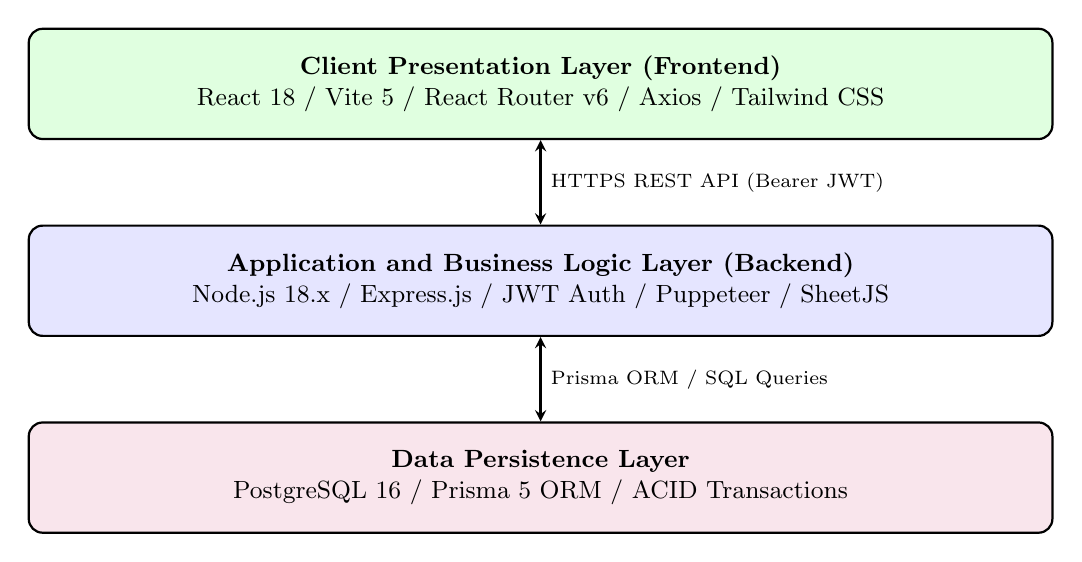
\begin{tikzpicture}[
  layer/.style={draw, thick, rounded corners=5pt,
    minimum width=13cm, minimum height=1.4cm,
    align=center, font=\small},
  arr/.style={thick, <->, >=stealth}
]
\node[layer, fill=green!12] (fe) at (0, 0)
    {\textbf{Client Presentation Layer (Frontend)}\\
     React 18 / Vite 5 / React Router v6 / Axios / Tailwind CSS};

\node[layer, fill=blue!10] (be) at (0,-2.5)
    {\textbf{Application and Business Logic Layer (Backend)}\\
     Node.js 18.x / Express.js / JWT Auth / Puppeteer / SheetJS};

\node[layer, fill=purple!10] (db) at (0,-5.0)
    {\textbf{Data Persistence Layer}\\
     PostgreSQL 16 / Prisma 5 ORM / ACID Transactions};

\draw[arr] (fe) -- node[right,font=\scriptsize]{HTTPS REST API (Bearer JWT)} (be);
\draw[arr] (be) -- node[right,font=\scriptsize]{Prisma ORM / SQL Queries} (db);
\end{tikzpicture}
\caption{Three-Tier System Architecture of TPMS}
\label{fig:arch}
\end{figure}

\section{System Design and Modules}
To ensure maintainability, scalability, and clean separation of concerns, TPMS is structured into cohesive functional modules. Each module encapsulates specific business logic and provides defined interfaces for user interaction and data processing:

\subsection{Authentication and Access Control Module}
This module manages secure user authentication and authorization across the platform. It handles user login, password hashing using modern cryptographic standards, stateless JSON Web Token (JWT) issuance and verification, and role-based route protection. The module enforces the five-role hierarchy (Student, Supervisor, External Examiner, Program Coordinator, and Maintainer) and ensures program-scoped data isolation between undergraduate and graduate departments.

\subsection{Group Formation and Project Registration Module}
This module governs the initiation of the project lifecycle. Coordinators publish academic project announcements with defined deadlines and team size constraints. Undergraduate students use this module to create project groups, send peer invitations via university roll numbers, and submit project proposals and research cluster choices. For graduate programs, it facilitates individual thesis topic and proposal registration.

\subsection{Coordinator Management and Faculty Allocation Module}
This module provides department coordinators with a centralized dashboard to manage submissions in real time. It features a deduplicated response matrix displaying complete team rosters, proposal details, and research domains. Coordinators use this module to assign supervisors, designate external defense examiners, and enforce conflict-of-interest rules that prevent faculty from examining projects they supervise.

\subsection{Document and Submission Management Module}
This module provides structured document handling for all project deliverables throughout the semester. It enables students to upload proposal manuscripts, mid-term progress reports, and final thesis documents. Supervisors and coordinators can review submissions, provide actionable feedback, and track submission statuses without relying on scattered physical copies or email attachments.

\subsection{Evaluation and Mark Calculation Module}
This module implements the official departmental grading rubrics for Minor projects (50 marks), Major projects (100 marks), and Master theses (300 marks). It provides an interactive criteria-wise mark entry interface for supervisors and examiners. The module automatically computes total marks, enforces maximum score boundaries, converts numerical scores into words, and prevents unauthorized modification of finalized defense results.

\subsection{Automated Report and PDF Generation Module}
This module dynamically compiles database records into standardized, print-ready A4 PDF evaluation sheets conforming to official university formats. It supports single-group downloads as well as bulk multi-project exports, enabling coordinators to instantly generate complete evaluation packages for examination archives.

\subsection{Bulk Data Ingestion and Notification Module}
This module simplifies large-scale departmental administration through automated data onboarding and communication. It provides a spreadsheet import engine capable of validating student rosters, checking for duplicate entries, and batch-creating user accounts. In addition, an asynchronous notification worker dispatches automated email updates to students and faculty regarding supervisor allocations, feedback availability, and defense schedules.

\section{Technology Stack}
\begin{table}[H]
\centering
\caption{Technology Stack and Justification}
\label{tab:tech_stack}
\vspace{4pt}
\small
\begin{tabularx}{\textwidth}{@{}l p{4.2cm} X@{}}
\toprule
\textbf{Layer} & \textbf{Technology} & \textbf{Justification} \\
\midrule
Frontend       & React 18 / Vite 5       & Component-based SPA with fast build tooling and reactive rendering \\
               & React Router v6         & Client-side role-guarded routing and protected page views \\
               & Tailwind CSS            & Utility-first responsive styling and layout design \\
\midrule
Backend        & Node.js 18+ / Express.js & Non-blocking I/O runtime and modular HTTP REST API framework \\
               & Puppeteer Core          & Headless browser engine for server-side A4 PDF grade sheet compilation \\
               & SheetJS (xlsx)          & Spreadsheet parser for roster validation and bulk account creation \\
               & bcryptjs / jsonwebtoken & Cryptographic password hashing and stateless token management \\
               & Nodemailer              & SMTP mail transport client for automated email notifications \\
\midrule
Database       & PostgreSQL 16           & Enterprise-grade relational DBMS with ACID compliance \\
               & Prisma 5 ORM            & Type-safe database client with declarative schema migrations \\
\bottomrule
\end{tabularx}
\end{table}

\section{Development Methodology}
The project adopted the \textbf{Prototyping Model} to accommodate evolving departmental requirements and ensure close alignment with stakeholder expectations. The development workflow was carried out through the following structured stages:

\begin{itemize}
  \item \textbf{Requirement Elicitation and Analysis:} Functional and non-functional requirements were gathered through discussions with the project supervisor, program coordinators, and student peers to identify essential academic workflows and evaluation guidelines.
  
  \item \textbf{Prototype Design and Development:} Initial user interface wireframes and interactive mockups were created for core components, including role-based dashboards, proposal registration forms, and defense evaluation scorecards.
  
  \item \textbf{Stakeholder Evaluation and Feedback:} The preliminary prototypes were presented to the project supervisor and departmental coordinators for review, identifying workflow bottlenecks, UI improvements, and validation rules early in the process.
  
  \item \textbf{Iterative Refinement and System Implementation:} Feedback from review sessions was incorporated into successive development iterations, transitioning the prototypes into fully functional frontend interfaces connected to backend business logic and the database.
  
  \item \textbf{System Testing and Integration:} Completed modules underwent functional verification, data consistency checks, and user acceptance testing across simulated defense workflows to prepare the platform for deployment.
\end{itemize}

\section{Data Handling}
In the current implementation, all persistent system data and uploaded documents are stored and managed within the local server environment:

\begin{itemize}
  \item \textbf{Local Relational Database Storage:} All structured application records, including user credentials, role allocations, project group compositions, defense evaluations, and audit events, are persisted in a local PostgreSQL relational database managed via Prisma ORM. Queries are executed through parameterized statements, preventing SQL injection and maintaining strict relational integrity.
  
  \item \textbf{Local Filesystem Document Storage:} Uploaded project proposals, progress reports, and generated A4 PDF evaluation sheets are stored directly on the local server filesystem within a dedicated storage directory (\texttt{/storage}), categorized by degree program and academic cohort.
  
  \item \textbf{Input Validation and Sanitization:} Client inputs received through RESTful endpoints undergo server-side validation. Uploaded document files are restricted to PDF format and verified for size constraints before being written to local storage.
  
  \item \textbf{Password Security:} User passwords are encrypted using bcrypt with salt rounds before being stored in the database, ensuring that plaintext passwords are never recorded.
\end{itemize}

\section{Testing and Validation}
To ensure functional correctness, data integrity, and system reliability, testing was conducted across three distinct phases:

\begin{itemize}
  \item \textbf{Unit Testing:} Individual controller functions, authentication middleware, validation logic, and mark calculation algorithms were tested in isolation to verify correct output across standard and edge-case inputs.
  
  \item \textbf{Integration Testing:} End-to-end API workflows spanning multiple system modules, such as team creation, document submission, coordinator approval, defense mark tabulation, and PDF compilation, were tested to ensure seamless inter-module communication.
  
  \item \textbf{User Acceptance Testing (UAT):} Representative stakeholders, including program coordinators, faculty supervisors, and students, tested the system against structured task scenarios to evaluate user interface responsiveness, workflow clarity, and overall operational readiness.
\end{itemize}

\section{Deployment Setup}
The platform is fully configured and executed within a \textbf{local server deployment} for system evaluation and departmental demonstration:

\begin{itemize}
  \item \textbf{Local Application Servers:} The backend REST API service runs locally on Node.js (port 5000), while the React frontend application is served locally via the Vite server (port 5173).
  
  \item \textbf{Local Database Service:} A local PostgreSQL database instance (port 5432) hosts the application schemas and relations, with database migrations applied through the Prisma CLI.
  
  \item \textbf{Local File Management:} Document uploads and downloads are handled directly via Node.js file system streams accessing the local storage directory.
  
  \item \textbf{SMTP Email Integration:} Automated email notifications for milestone events, supervisor assignments, and defense feedback are dispatched through an integrated SMTP (Simple Mail Transfer Protocol) transport service, configured via local environment parameters.
  
  \item \textbf{Environment Security:} All local configurations, including database connection strings, JWT signing keys, and SMTP server credentials, are isolated in a root-level \texttt{.env} file.
\end{itemize}

\chapter{Implementation Details}

\section{Requirements Specification}

\subsection{Functional Requirements}
The functional requirements of the Thesis and Project Management System (TPMS) define the specific operations, behaviors, and services the platform provides to its users. Table~\ref{tab:fr} summarizes the functional requirements categorized by system module.

\begin{table}[H]
\centering
\caption{Functional Requirements of TPMS}
\label{tab:fr}
\vspace{4pt}
\small
\begin{tabularx}{\textwidth}{@{}l p{3.2cm} X@{}}
\toprule
\textbf{Req ID} & \textbf{Module} & \textbf{Requirement Description} \\
\midrule
\textbf{FR-01} & Authentication & The system shall authenticate users and enforce Role-Based Access Control (RBAC) across all user roles. \\

\textbf{FR-02} & Announcements & Coordinators shall be able to publish project and thesis announcements with defined parameters and deadlines. \\

\textbf{FR-03} & Project Registration & Students shall be able to form project teams by inviting peers and submit project proposals. \\

\textbf{FR-04} & Faculty Allocation & Coordinators shall be able to assign faculty supervisors and designate defense examiners. \\

\textbf{FR-05} & Document Management & Students shall be able to upload project reports, and faculty shall be able to view and review submissions. \\

\textbf{FR-06} & Defense Evaluation & Evaluators shall be able to enter criteria-wise marks based on departmental scoring rubrics. \\

\textbf{FR-07} & Report \& PDF Export & The system shall automatically compute total marks and generate official, print-ready A4 PDF evaluation sheets. \\

\textbf{FR-08} & Bulk Data Import & Coordinators shall be able to onboard student rosters in bulk via structured Excel spreadsheets. \\
\bottomrule
\end{tabularx}
\end{table}

\subsection{Non-Functional Requirements}
The non-functional requirements define the quality attributes, usability standards, and security constraints of the system:

\begin{itemize}
  \item \textbf{Security:} User passwords must be securely hashed using bcrypt before storage, and API routes must be protected using token-based authentication (JWT). All database queries must be parameterized to safeguard against SQL injection.
  
  \item \textbf{Usability:} The user interface must be clean, responsive, and easy to navigate, providing dedicated dashboards tailored to each user role (Student, Supervisor, Coordinator).
  
  \item \textbf{Data Integrity and Reliability:} The system must maintain data consistency across all project records, preventing duplicate entries and validating inputs before database operations.
  
  \item \textbf{Modularity and Maintainability:} The system must follow a modular architecture separating frontend components, backend logic, and database schemas to facilitate future updates and maintenance.
  
  \item \textbf{Compatibility:} The web application must be compatible with standard modern web browsers (e.g., Google Chrome, Mozilla Firefox, Microsoft Edge) without requiring third-party browser extensions.
\end{itemize}

\section{System Overview}
The implementation of TPMS maps the architectural specifications established in Chapter 3 into a decoupled, three-tier software application. The presentation layer is structured as a component-driven React Single-Page Application (SPA), the application tier is organized into modular Express.js controllers and services, and the persistence layer is modeled in a PostgreSQL relational database managed by Prisma ORM.

Figure~\ref{fig:usecase} illustrates the comprehensive Use Case Diagram of the system, depicting the core functional interactions accessible to each user role: Students, Supervisors, Program Coordinators, External Examiners, and Department Maintainers.

\begin{figure}[H]
\centering
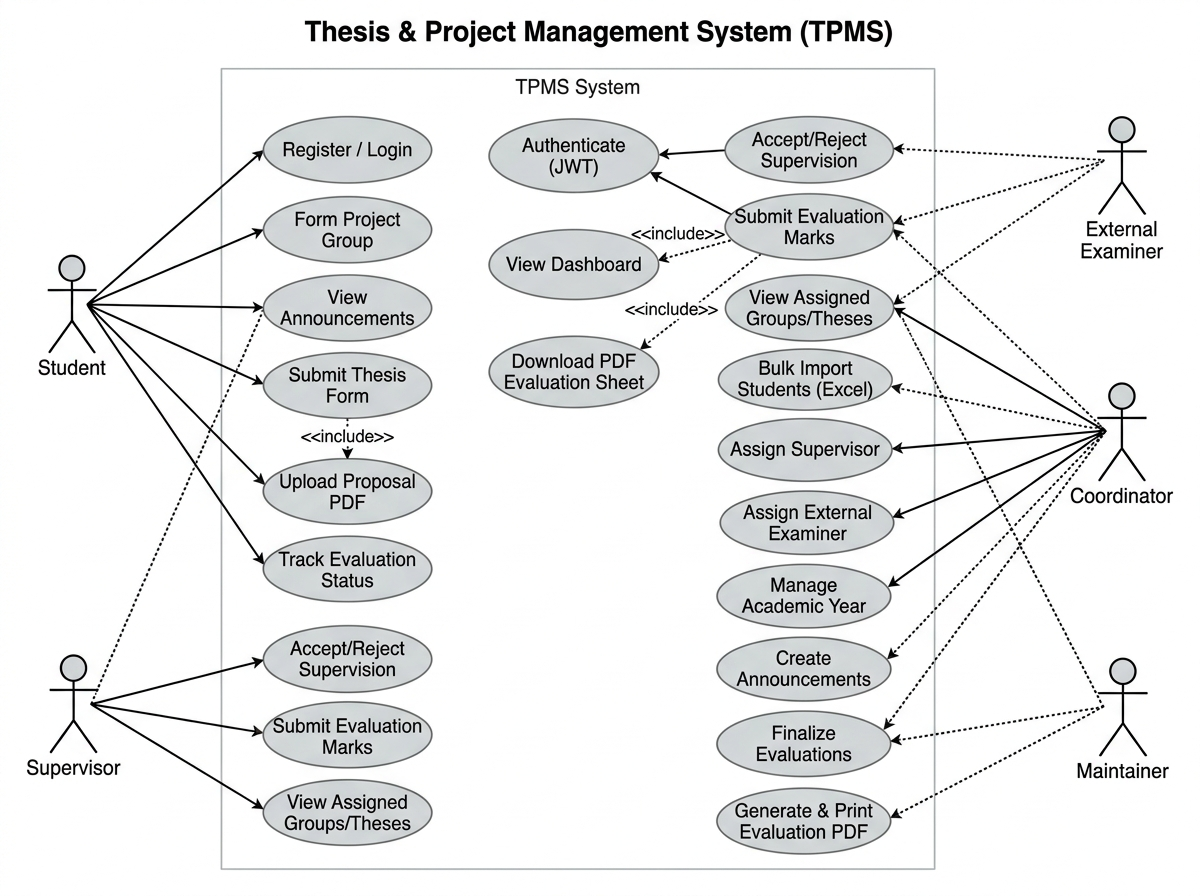
\includegraphics[width=0.96\textwidth]{fig_usecase.jpg}
\caption{Use Case Diagram of TPMS Across All User Roles}
\label{fig:usecase}
\end{figure}

The five principal actors interact with the system as follows:
\begin{itemize}
  \item \textbf{Students:} Create project groups or register thesis topics, invite team members, submit proposal documents, and track evaluation milestones.
  \item \textbf{Supervisors:} Review assigned project proposals, provide document feedback, and submit mid-term and final defense evaluation marks.
  \item \textbf{External Examiners:} Access assigned defense dossiers and record criteria-wise scores during defense sessions.
  \item \textbf{Program Coordinators:} Manage batch announcements, perform bulk student onboarding, allocate supervisors and examiners with conflict-of-interest checks, and export composite PDF grade sheets.
  \item \textbf{Department Maintainers:} Oversee global department configurations, academic degree programs, and system audit logs.
\end{itemize}

\section{Development Environment}
The development of TPMS was carried out across a collaborative team environment utilizing standard open-source tools, modern web runtimes, and a relational database. Table~\ref{tab:dev_env} summarizes the hardware, software, and development specifications used during the implementation.

\begin{table}[H]
\centering
\caption{Development Environment Specifications}
\label{tab:dev_env}
\vspace{4pt}
\small
\begin{tabularx}{\textwidth}{@{}l p{4.2cm} X@{}}
\toprule
\textbf{Category} & \textbf{Component / Tool} & \textbf{Specification / Details} \\
\midrule
\textbf{Operating System} & Development Platforms & Fedora Linux / Microsoft Windows 11 (64-bit) \\

\textbf{Frontend Stack} & UI Library \& Build Tool & React 18.2.0, Vite 5.1.0, Tailwind CSS \\
 & Routing \& State Management & React Router DOM 6.22, Axios HTTP Client \\
 & Icons \& UI Components & Lucide React, Recharts \\

\textbf{Backend Stack} & Runtime \& Framework & Node.js (v18+), Express.js 4.18.2 \\
 & Security \& Authentication & JSON Web Token (JWT), bcryptjs, Helmet \\
 & Email Service & Nodemailer (SMTP Transport) \\
 & Document Processing & SheetJS (xlsx), PDFKit, Puppeteer Core \\

\textbf{Database \& ORM} & Database Engine & PostgreSQL 16 \\
 & Object-Relational Mapping & Prisma ORM 5.10.0 (with automated migrations) \\

\textbf{Tooling \& Versioning} & Code Editor / IDE & Visual Studio Code \\
 & API Testing \& Inspection & Postman / REST Client, Prisma Studio \\
 & Version Control & Git with GitHub Remote Repository \\
\bottomrule
\end{tabularx}
\end{table}

\section{System Implementation}

\subsection{Database Schema Design}
The TPMS persistence layer is implemented in PostgreSQL using Prisma ORM. The relational model consists of 14 normalized tables that manage users, academic programs, student groups, proposals, supervisor assignments, and evaluation records while enforcing strict foreign-key constraints. Figure~\ref{fig:er} illustrates the complete Entity-Relationship (ER) Diagram of the database.

\begin{figure}[H]
\centering
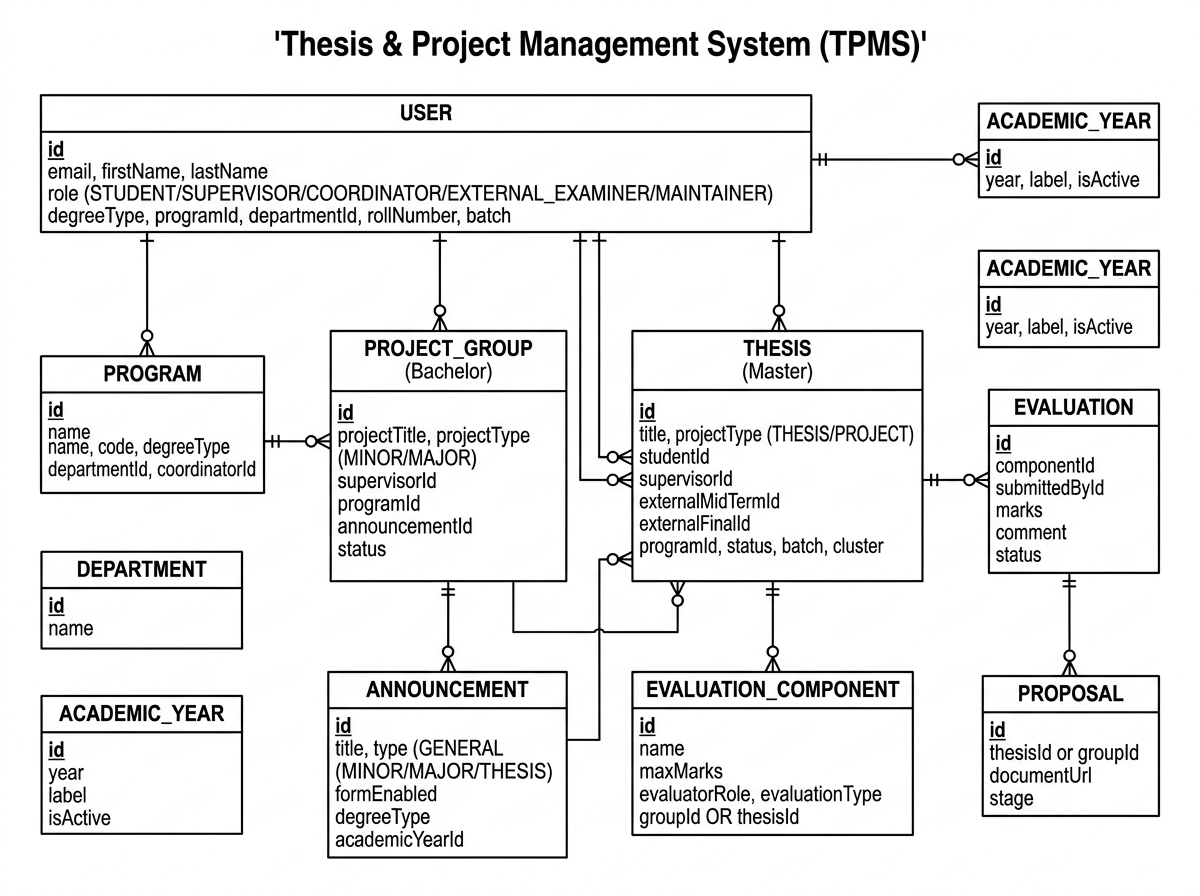
\includegraphics[width=0.97\textwidth]{fig_er.jpg}
\caption{Entity-Relationship (ER) Diagram of TPMS Database}
\label{fig:er}
\end{figure}

Key data dictionary specifications for primary application tables are provided in Tables~\ref{tab:user_dd} and \ref{tab:group_dd}.

\begin{table}[H]
\centering
\caption{Data Dictionary: \texttt{User} Table}
\label{tab:user_dd}
\vspace{4pt}
\small
\begin{tabularx}{\textwidth}{@{}l l l X@{}}
\toprule
\textbf{Field Name} & \textbf{Data Type} & \textbf{Constraint} & \textbf{Description} \\
\midrule
\texttt{id}          & SERIAL    & Primary Key   & Unique identifier for the user account. \\
\texttt{email}       & VARCHAR   & UNIQUE, NOT NULL & Institutional email address (\texttt{@pcampus.edu.np}). \\
\texttt{password}    & VARCHAR   & NOT NULL      & bcrypt hashed password string. \\
\texttt{name}        & VARCHAR   & NOT NULL      & Full name of the student or faculty member. \\
\texttt{role}        & ENUM      & NOT NULL      & Assigned role (Student, Supervisor, Coordinator, etc.). \\
\texttt{rollNumber}  & VARCHAR   & Nullable      & University roll number for student accounts. \\
\texttt{programId}   & INTEGER   & Foreign Key   & References the associated degree program. \\
\bottomrule
\end{tabularx}
\end{table}

\begin{table}[H]
\centering
\caption{Data Dictionary: \texttt{ProjectGroup} Table}
\label{tab:group_dd}
\vspace{4pt}
\small
\begin{tabularx}{\textwidth}{@{}l l l X@{}}
\toprule
\textbf{Field Name} & \textbf{Data Type} & \textbf{Constraint} & \textbf{Description} \\
\midrule
\texttt{id}              & SERIAL  & Primary Key   & Unique identifier for the project team. \\
\texttt{projectTitle}    & VARCHAR & NOT NULL      & Approved title of the Bachelor project. \\
\texttt{projectType}     & ENUM    & DEFAULT: MINOR & Project tier (\texttt{MINOR} or \texttt{MAJOR}). \\
\texttt{status}          & ENUM    & DEFAULT: PENDING & Lifecycle status (\texttt{PENDING}, \texttt{ACTIVE}, \texttt{COMPLETED}). \\
\texttt{supervisorId}    & INTEGER & Foreign Key   & References the assigned faculty supervisor. \\
\texttt{programId}       & INTEGER & Foreign Key   & References the owning department program. \\
\texttt{academicYearId}  & INTEGER & Foreign Key   & References the active academic year batch. \\
\bottomrule
\end{tabularx}
\end{table}

\subsection{Data Flow Architecture}
The flow of information across user roles, backend API services, and database tables is modeled using Data Flow Diagrams. Figure~\ref{fig:dfd} presents the Level-1 Data Flow Diagram (DFD) showing how inputs from students, faculty, and coordinators traverse the core authentication, group registration, allocation, and evaluation processes.

\begin{figure}[H]
\centering
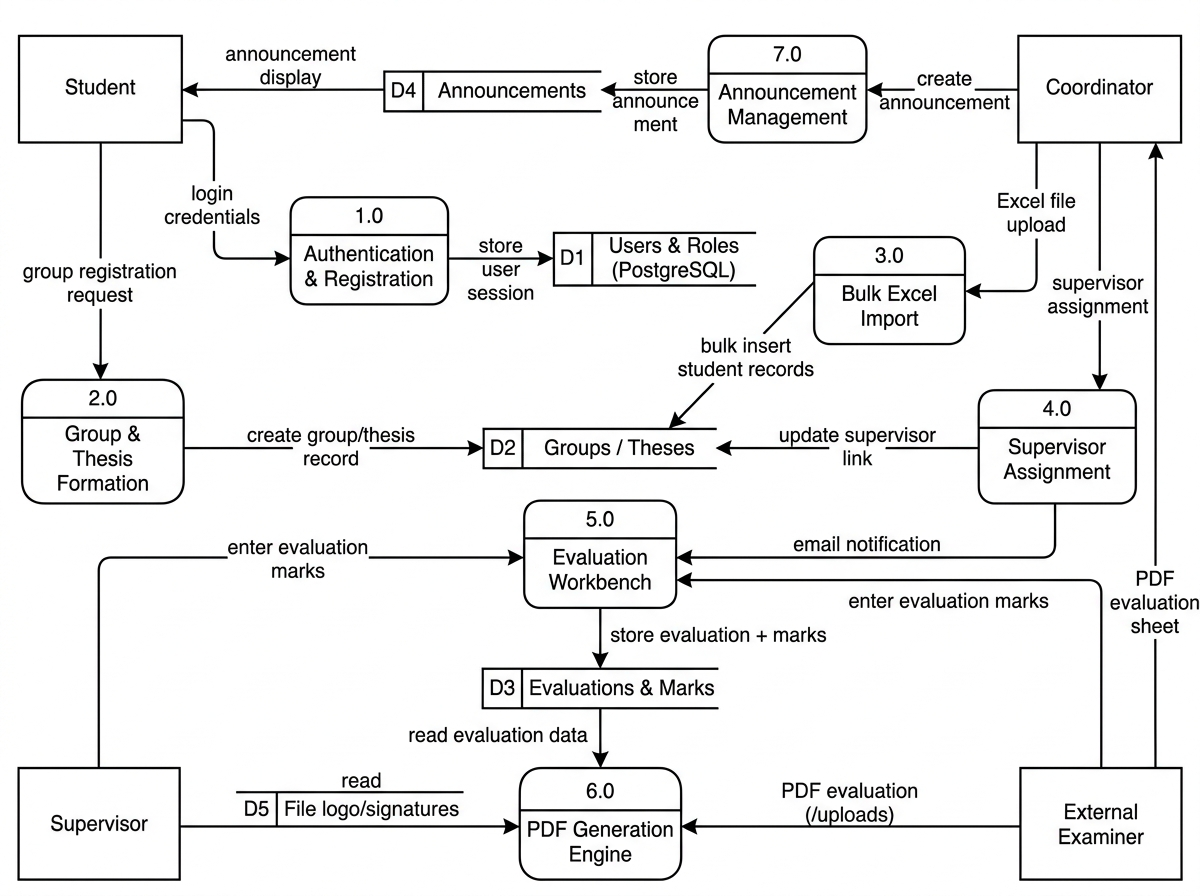
\includegraphics[width=0.97\textwidth]{fig_dfd.jpg}
\caption{Data Flow Diagram (DFD Level 1) of TPMS}
\label{fig:dfd}
\end{figure}

The diagram identifies core processes: User Authentication, Group and Thesis Registration, Bulk Excel Ingestion, Supervisor Allocation, Defense Evaluation, and PDF Generation, supported by structured database data stores.

\subsection{Bulk Student Data Onboarding Pipeline}
To avoid manual account creation for large student batches, TPMS provides a spreadsheet ingestion pipeline. Coordinators upload structured class rosters in \texttt{.xlsx} format. The system parses the spreadsheet, validates column headers, checks for intra-file duplicate roll numbers, and verifies against existing database records. Clean records are batch-inserted in a single database transaction.

Figure~\ref{fig:seq_import} illustrates the sequence of interactions involved in the Excel bulk import workflow.

\begin{figure}[H]
\centering
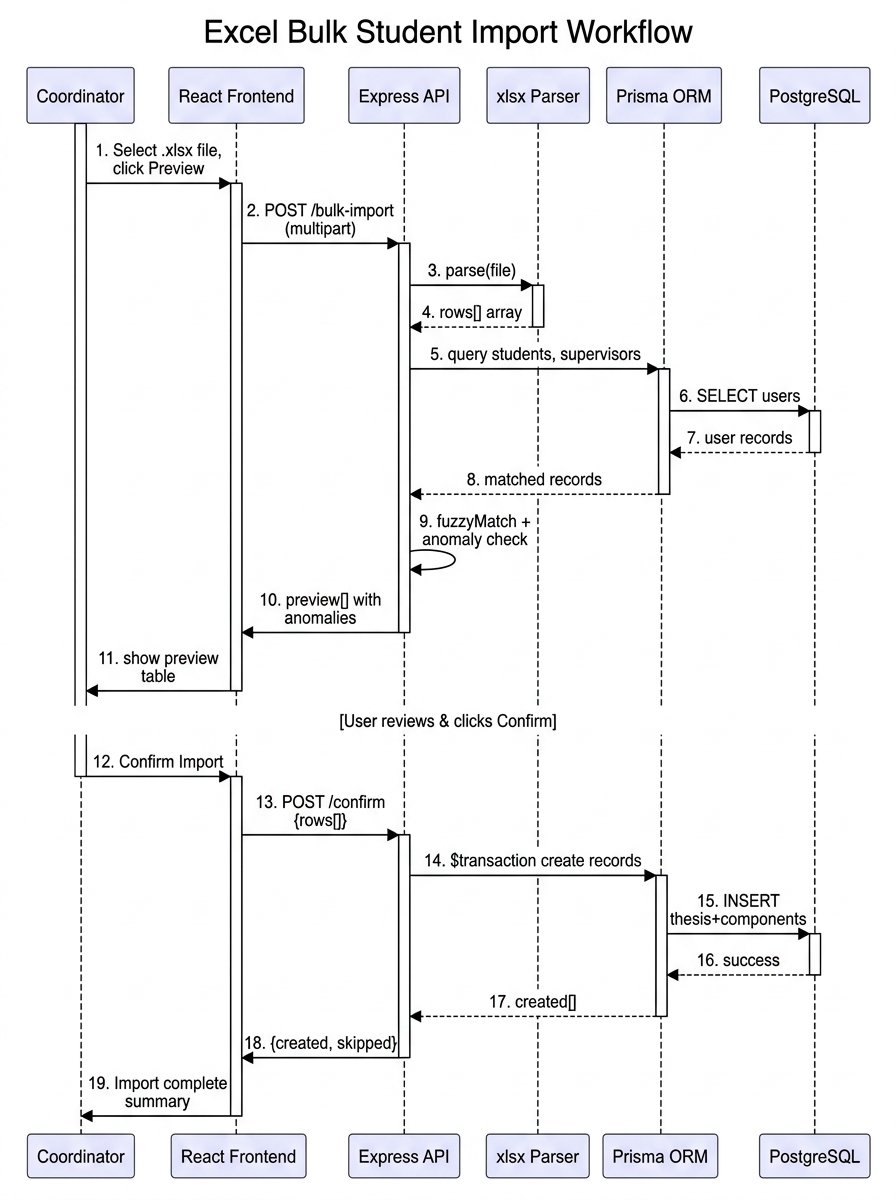
\includegraphics[width=0.95\textwidth]{fig_seq_import.jpg}
\caption{Sequence Diagram for Bulk Student Excel Onboarding}
\label{fig:seq_import}
\end{figure}

\subsection{Evaluation and PDF Generation Engine}
The evaluation engine supports multi-criteria defense scoring for Minor projects (50 marks), Major projects (100 marks), and Master theses (300 marks). Evaluators enter marks per criterion through an interactive interface. The system validates score limits, automatically computes aggregate marks, and converts total numerical scores to words to eliminate manual calculation errors.

Once marks are submitted, the system dynamically renders official, print-ready A4 PDF evaluation sheets directly from the database records. Figure~\ref{fig:seq_pdf} illustrates the sequence of interactions during mark submission and PDF compilation.

\begin{figure}[H]
\centering
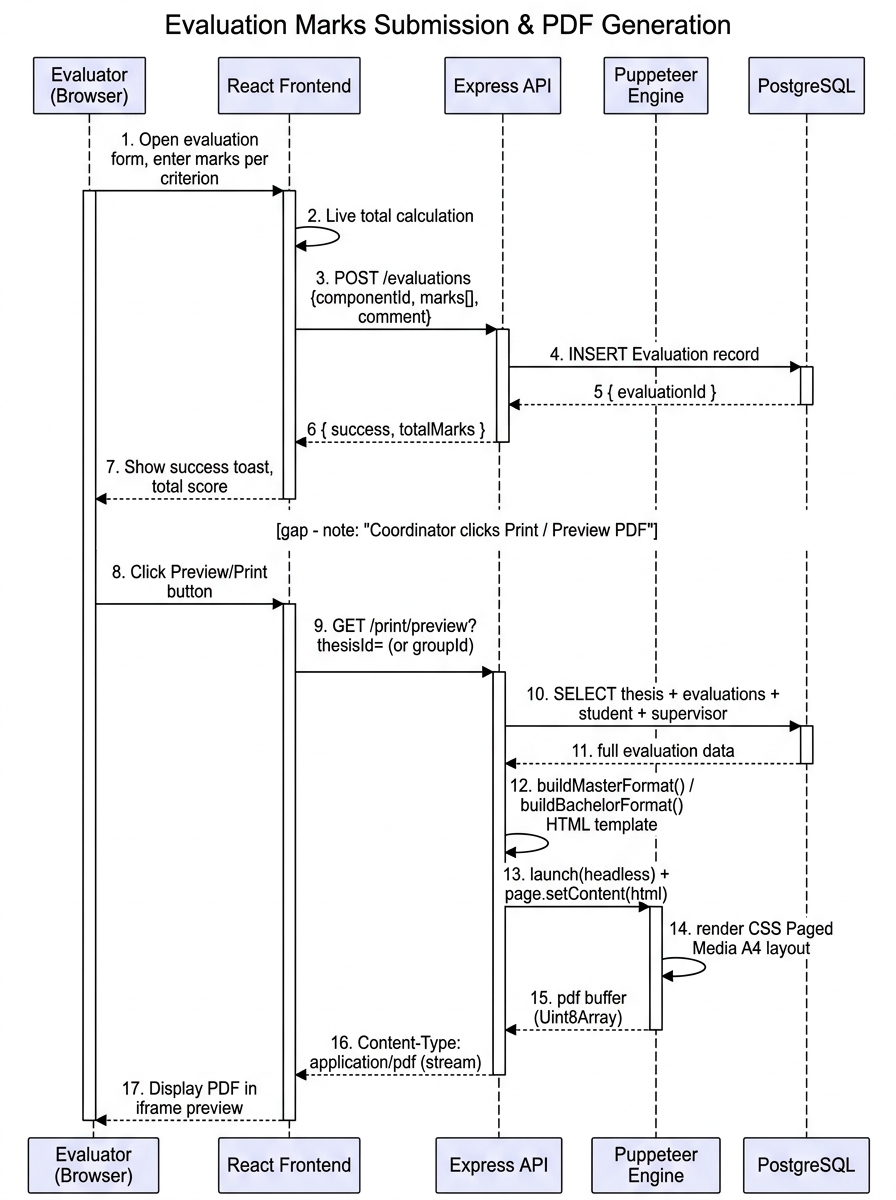
\includegraphics[width=0.95\textwidth]{fig_seq_pdf.jpg}
\caption{Sequence Diagram for Defense Evaluation and PDF Generation}
\label{fig:seq_pdf}
\end{figure}

\section{Interface and Visualization}
The frontend interface of TPMS is implemented as a responsive Single-Page Application (SPA) providing role-specific dashboards, interactive forms, and real-time status indicators across the primary user roles:

\begin{itemize}
  \item \textbf{Coordinator Management Interface:} Figure~\ref{fig:ui_coordinator} illustrates the coordinator response matrix, allowing program coordinators to monitor submitted projects, filter by academic batch, assign supervisors, and track project lifecycle statuses.
  
  \item \textbf{Student Project and Submission View:} Figure~\ref{fig:ui_student} depicts the student workspace, displaying project details, assigned faculty, research cluster domain, and multi-stage milestone submission tabs (Proposal, Mid-Term, Final).
  
  \item \textbf{Criteria-Wise Defense Evaluation Interface:} Figure~\ref{fig:ui_eval} demonstrates the defense scoring scorecard used by supervisors and external examiners to submit criteria-wise marks with real-time score calculation.
\end{itemize}

\begin{figure}[H]
\centering
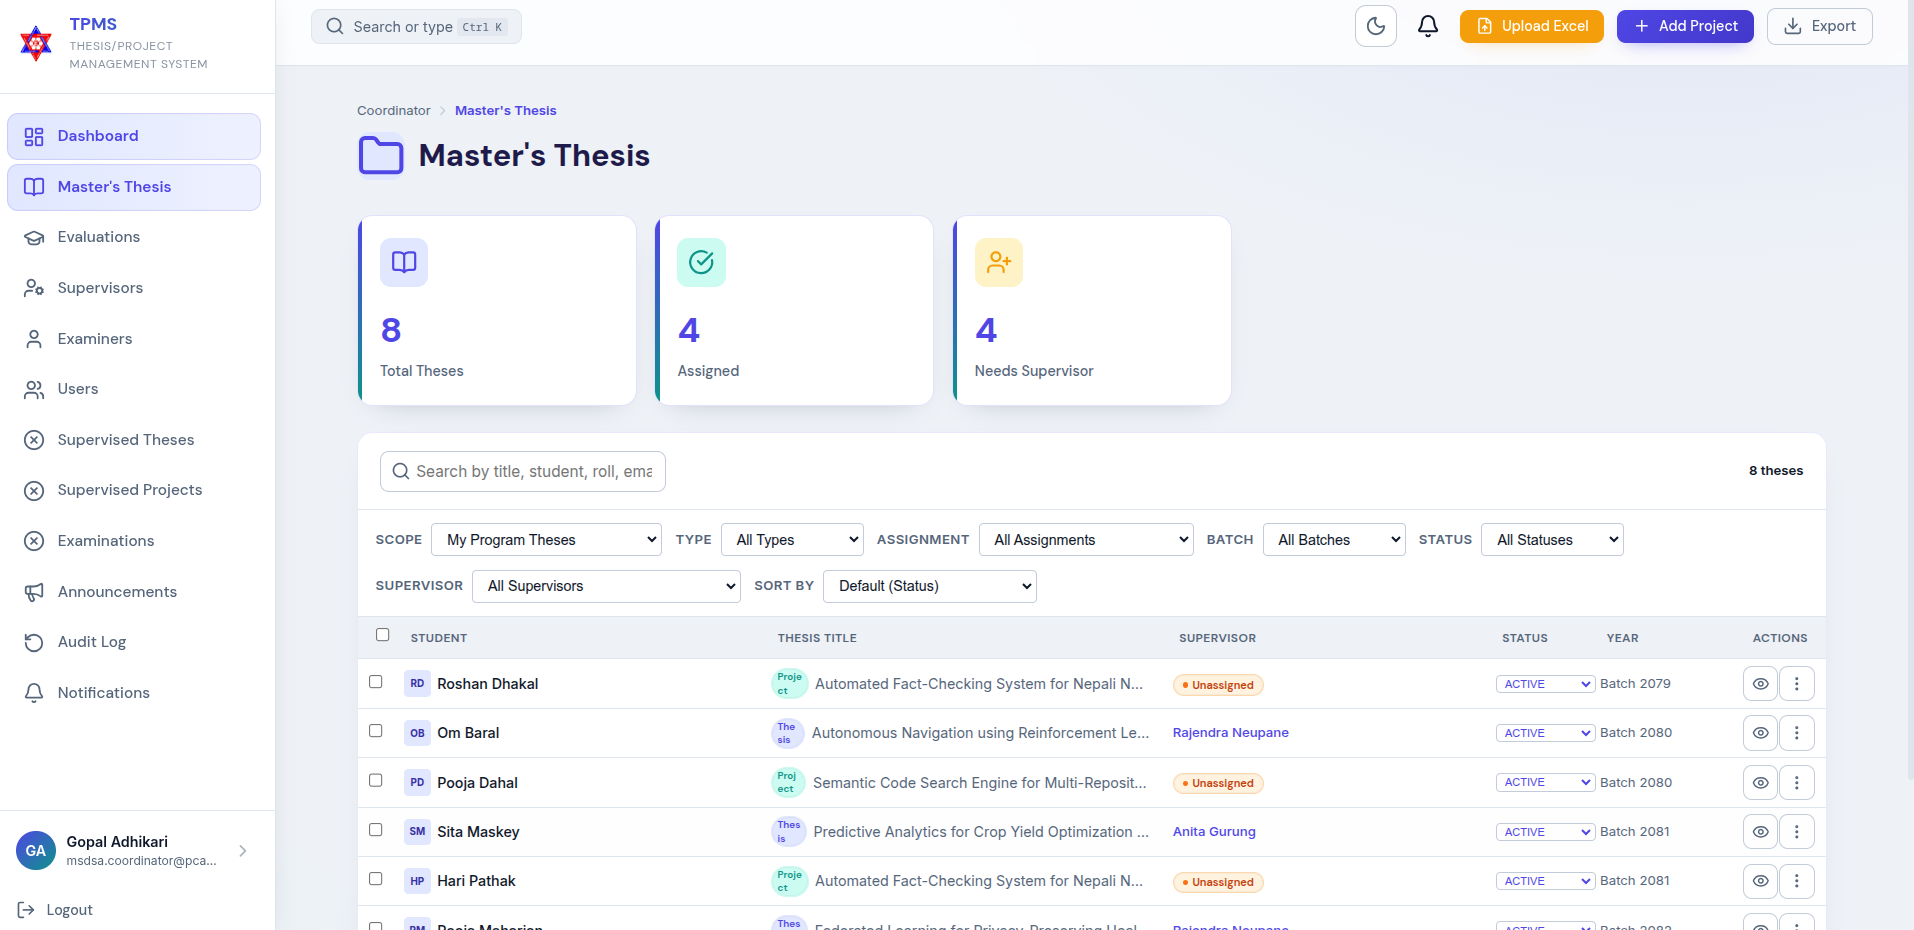
\includegraphics[width=0.95\textwidth]{project/project_page.png}
\caption{Coordinator Project Management and Allocation Interface}
\label{fig:ui_coordinator}
\end{figure}

\begin{figure}[H]
\centering
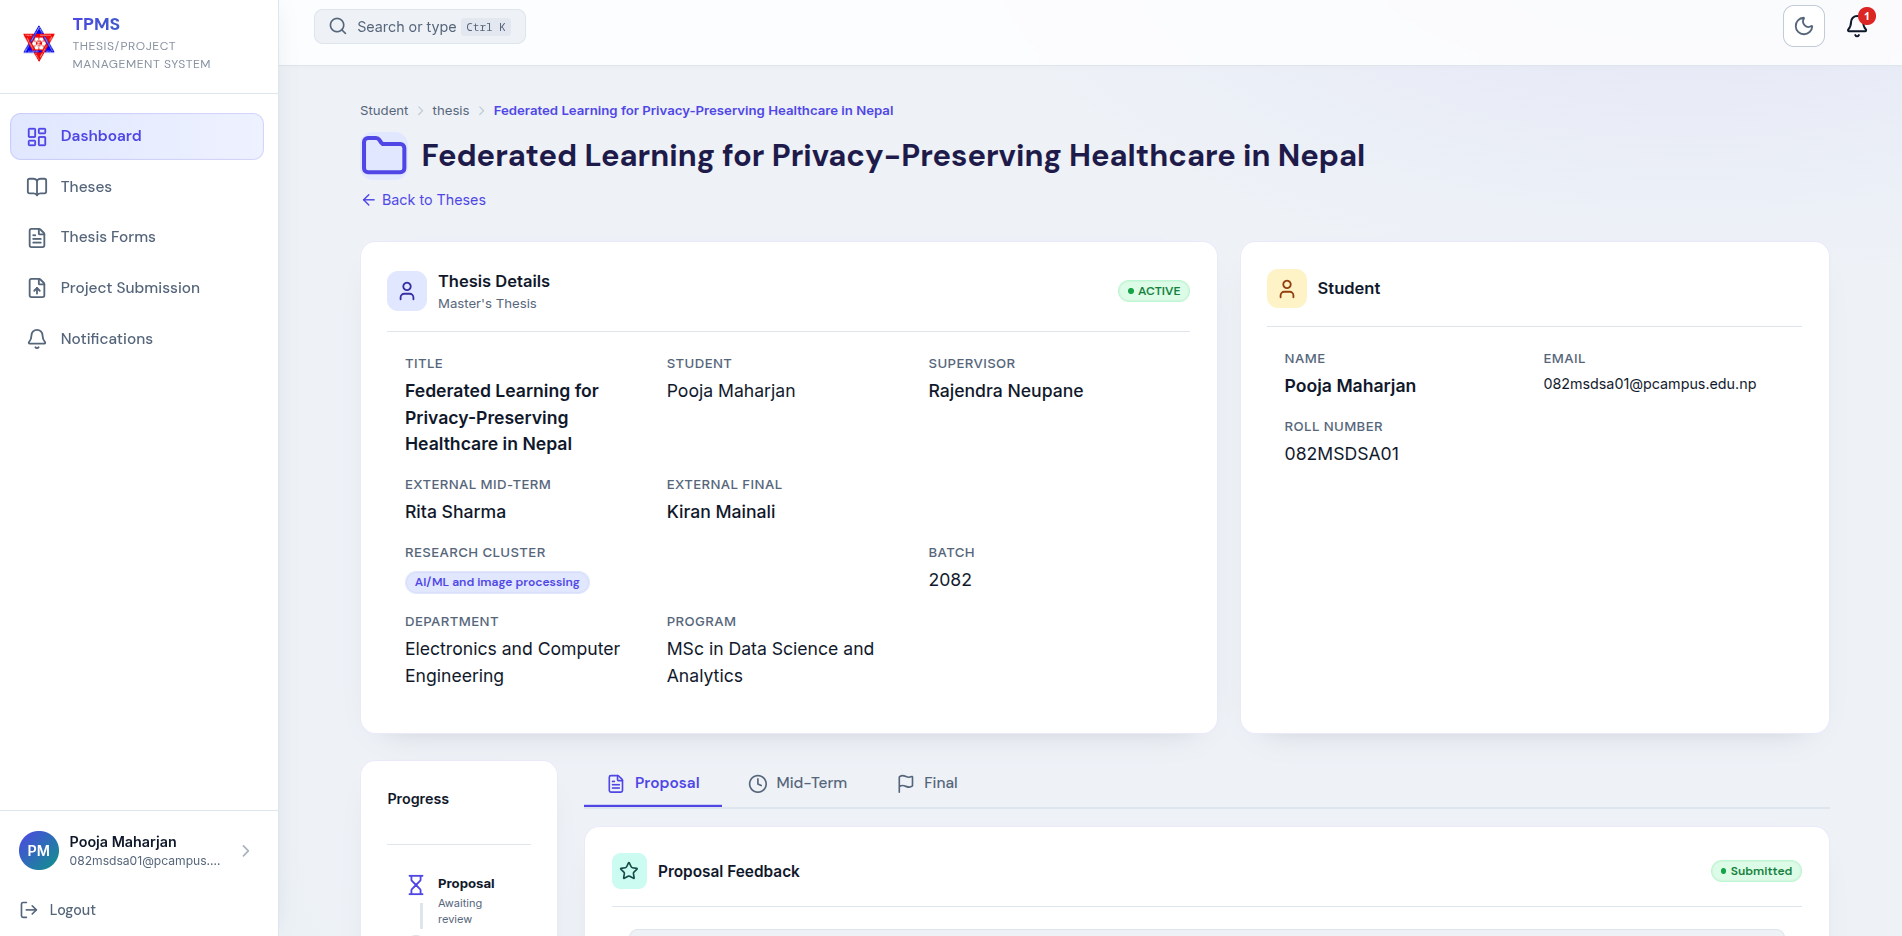
\includegraphics[width=0.95\textwidth]{project/student_project_page.png}
\caption{Student Project Details and Submission Progress Interface}
\label{fig:ui_student}
\end{figure}

\begin{figure}[H]
\centering
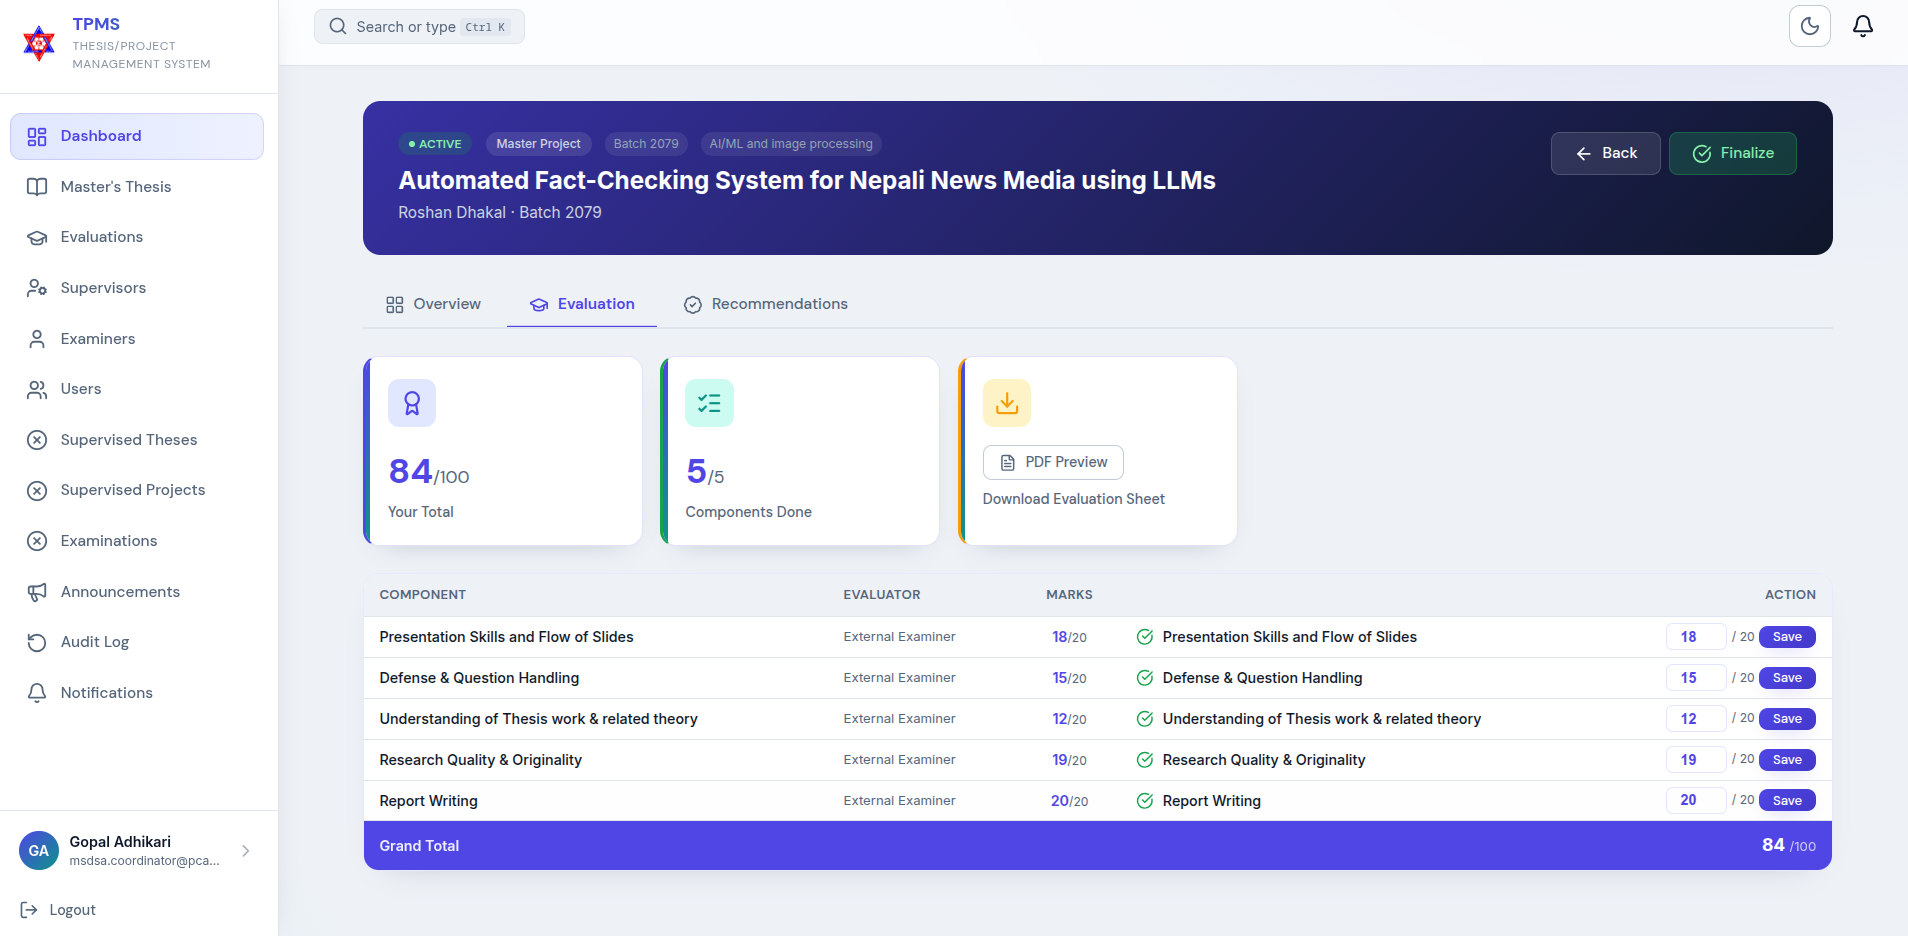
\includegraphics[width=0.95\textwidth]{project/evaluation_page.png}
\caption{Criteria-Wise Defense Evaluation and Score Entry Interface}
\label{fig:ui_eval}
\end{figure}

\section{Deployment and Execution}
The platform is fully configured and executed within a \textbf{local server environment (Localhost)} for testing and demonstration:

\begin{itemize}
  \item \textbf{Local Backend Runtime:} The Node.js Express server runs on port 5000, handling API requests, business logic execution, and background PDF compilation.
  
  \item \textbf{Local Frontend Runtime:} The React application is served locally via the Vite server on port 5173, communicating asynchronously with the backend API.
  
  \item \textbf{Local Database Service:} A local PostgreSQL database instance on port 5432 manages relational tables and migrations via Prisma ORM.
  
  \item \textbf{Local Storage Directory:} Uploaded proposal documents, progress reports, and generated A4 PDF evaluation sheets are stored in the local server storage directory (\texttt{/storage}).
  
  \item \textbf{SMTP Email Integration:} Automated email notifications are dispatched via an SMTP mail transport service configured through local environment variables.
\end{itemize}

\section{Challenges and Solutions}
During the system design and implementation phases, several technical challenges were encountered and successfully resolved, as summarized in Table~\ref{tab:challenges}.

\begin{table}[H]
\centering
\caption{Technical Challenges Encountered and Solutions Applied}
\label{tab:challenges}
\vspace{4pt}
\small
\begin{tabularx}{\textwidth}{@{}p{4.5cm} X@{}}
\toprule
\textbf{Technical Challenge} & \textbf{Applied Solution} \\
\midrule
Deduplicating multi-student group submissions in the coordinator dashboard & Implemented a database aggregation query that groups individual member entries by team ID and consolidates complete rosters into single rows. \\
\addlinespace
Automated conflict-of-interest prevention during examiner assignment & Built an algorithmic filter that checks project supervisor IDs and dynamically excludes the assigned supervisor from the eligible examiner list. \\
\addlinespace
Preventing concurrent double-enrollment across project teams & Implemented database-level validation checks (Engagement Guard) ensuring a student cannot hold multiple active project memberships. \\
\addlinespace
Standardized university-format PDF generation with word-equivalent marks & Utilized server-side HTML/CSS template compilation with an automated number-to-words algorithm to render official A4 evaluation sheets. \\
\bottomrule
\end{tabularx}
\end{table}

\chapter{Results and Discussion}

\section{Results}
The developed Thesis and Project Management System (TPMS) was thoroughly evaluated through functional workflow execution, document generation validation, and multi-level system testing.

\subsection{Functional Workflow Execution}
The platform successfully executed the complete project and thesis lifecycle across the Department of Electronics and Computer Engineering (DOECE):
\begin{itemize}
  \item \textbf{Team Formation and Proposal Submission:} Students successfully created project teams, invited group members via roll numbers, and submitted proposals. The duplicate enrollment check reliably prevented students from participating in multiple active groups.
  
  \item \textbf{Coordinator Allocation Matrix:} Coordinators accessed the centralized response matrix to filter submissions by cluster, assign project supervisors, and allocate defense examiners with automatic conflict-of-interest exclusion.
  
  \item \textbf{Bulk Roster Ingestion:} The spreadsheet import engine parsed class rosters, identified duplicate records during pre-import validation, and onboarded student cohorts in batch operations.
\end{itemize}

\subsection{Evaluation and PDF Generation Output}
The criteria-based evaluation engine was tested against departmental grading rubrics across all academic tiers (Minor: 50 marks, Major: 100 marks, Master Thesis: 300 marks). Evaluators entered marks per individual criterion, and the system automatically computed aggregate totals while enforcing upper score bounds.

Figure~\ref{fig:result_pdf} shows the evaluation review interface and the dynamically rendered official A4 PDF evaluation grade sheet, complete with institutional headers, criteria mark breakdown, and signature blocks.

\begin{figure}[H]
\centering
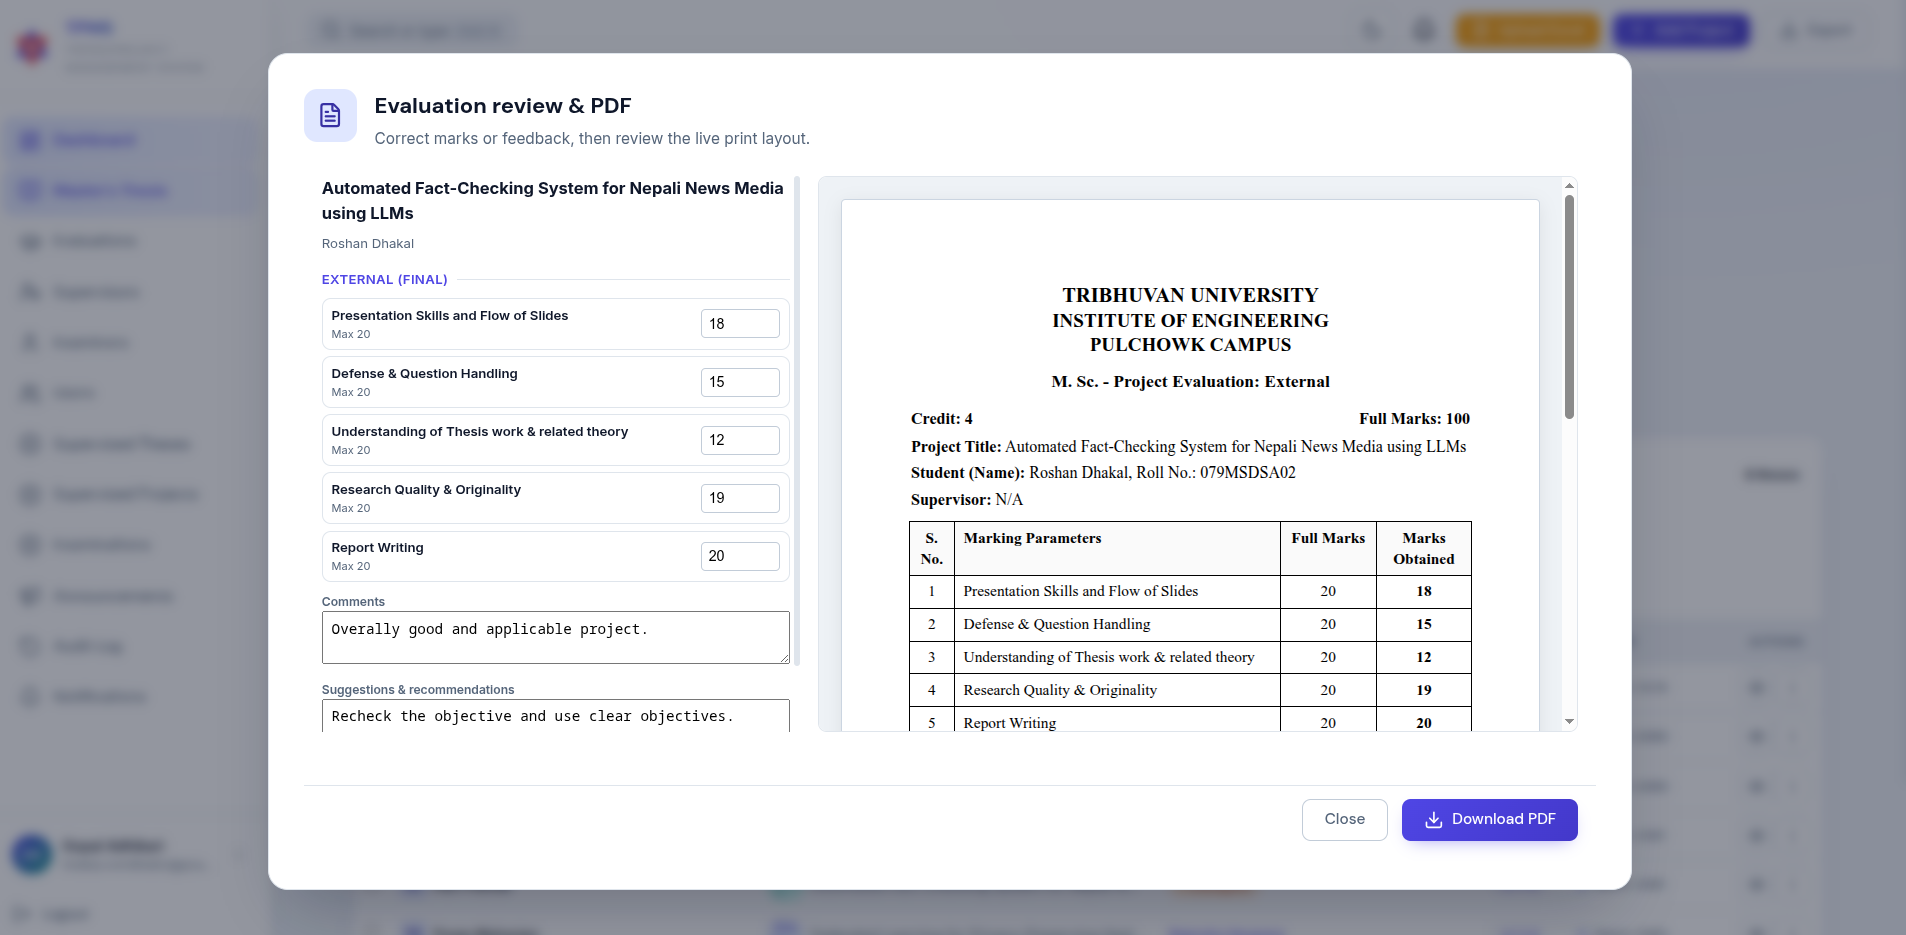
\includegraphics[width=0.95\textwidth]{project/pdf.png}
\caption{Live Evaluation Review and Official A4 PDF Grade Sheet Generation}
\label{fig:result_pdf}
\end{figure}

Figure~\ref{fig:result_analytics} illustrates the program overview dashboard, displaying batch statistics, thesis statuses, and actionable coordinator notifications.

\begin{figure}[H]
\centering
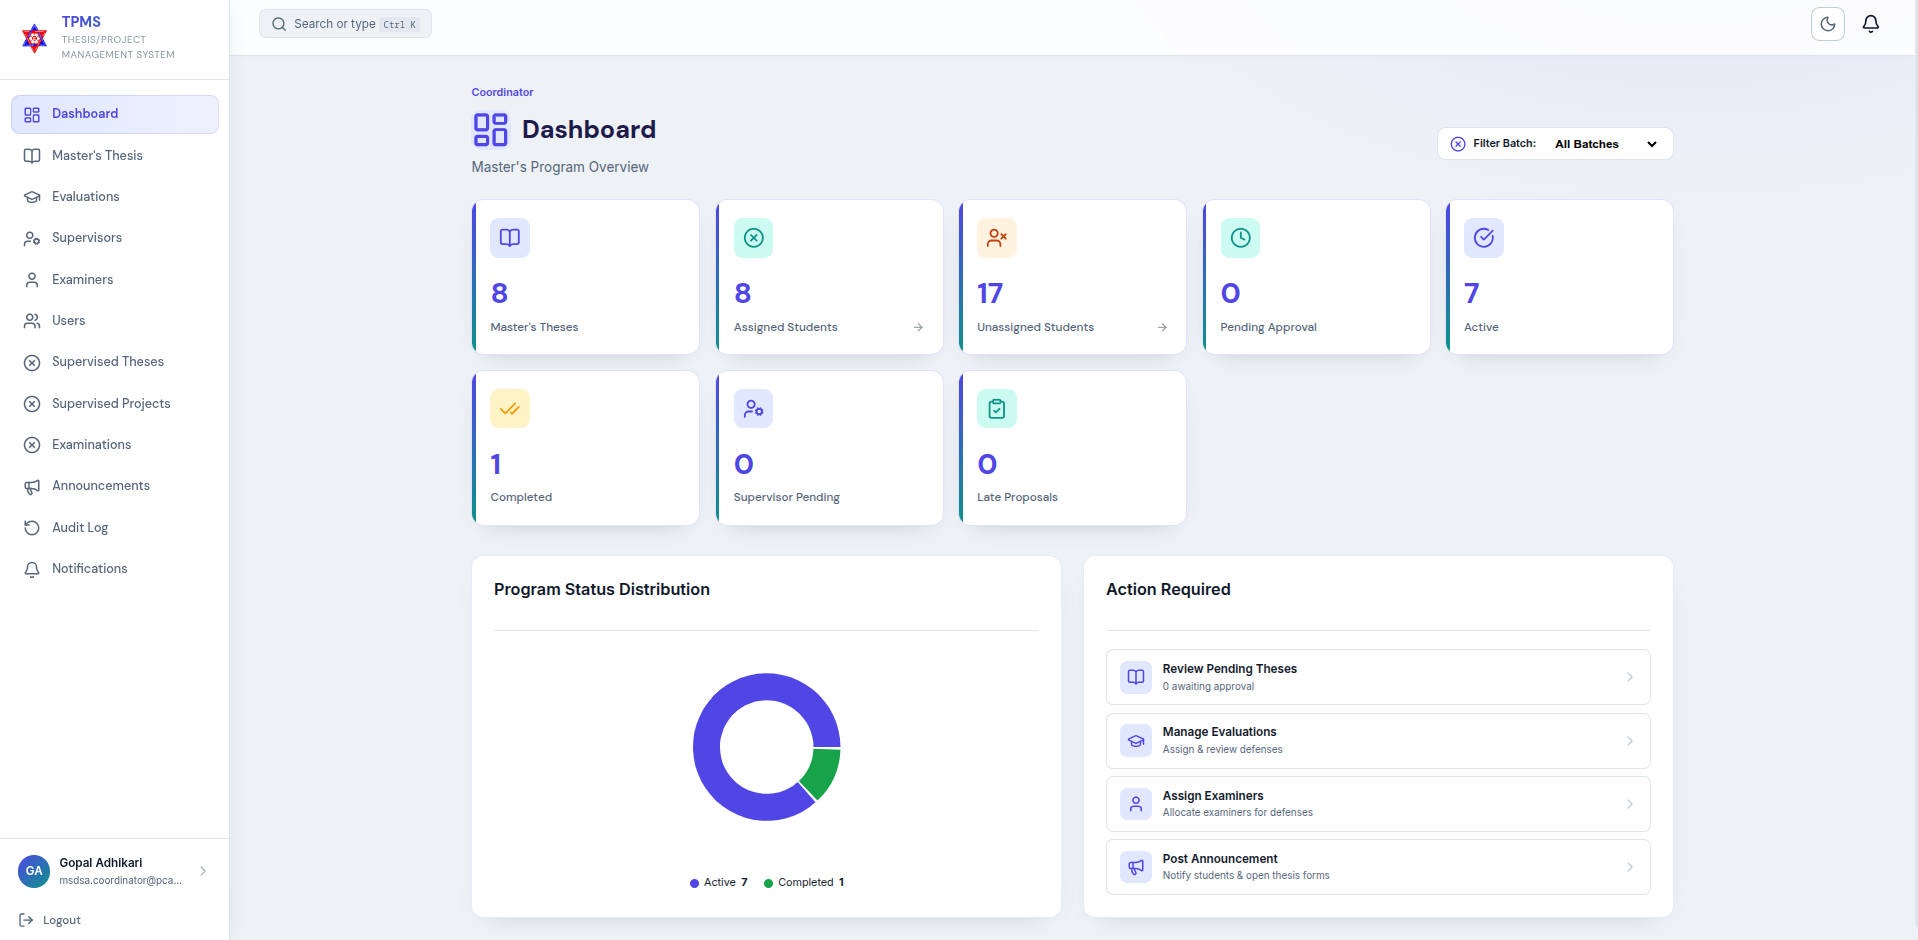
\includegraphics[width=0.95\textwidth]{project/dashboard.png}
\caption{Program Overview Analytics and Status Distribution Dashboard}
\label{fig:result_analytics}
\end{figure}

\subsection{System Verification and Testing Results}
System correctness and reliability were verified through structured testing phases:

\begin{itemize}
  \item \textbf{Unit and Component Testing:} Core utility functions, validation middleware, and mark calculation algorithms were tested across positive and negative cases. Table~\ref{tab:unit_tests} summarizes the testing outcomes across system modules.
\end{itemize}

\begin{table}[H]
\centering
\caption{System Module Testing Results}
\label{tab:unit_tests}
\vspace{4pt}
\small
\begin{tabularx}{\textwidth}{@{}l p{4.5cm} X c@{}}
\toprule
\textbf{Module} & \textbf{Verified Functionality} & \textbf{Test Scenario} & \textbf{Outcome} \\
\midrule
Authentication    & JWT token issuance \& route protection & Valid login, expired tokens, role checks & Pass \\
Group Formation   & Team invitation \& duplicate prevention & Member invite, double-enrollment block & Pass \\
Faculty Allocation& Supervisor \& examiner assignment & Assignment matrix, supervisor exclusion & Pass \\
Evaluation Engine & Criteria marks entry \& score sum & Boundary check, draft/final submit & Pass \\
PDF Compilation   & Dynamic A4 document generation & HTML-to-PDF render, words conversion & Pass \\
Bulk Import       & Excel roster validation & Header check, duplicate roll detection & Pass \\
\bottomrule
\end{tabularx}
\end{table}

\begin{itemize}
  \item \textbf{Integration and Security Testing:} End-to-end user workflows spanning team registration, supervisor assignment, mark compilation, and PDF generation executed seamlessly without data inconsistencies. Security tests confirmed that unauthenticated requests and role escalation attempts were blocked with appropriate HTTP status codes.
  
  \item \textbf{User Acceptance Testing (UAT):} Department coordinators, faculty supervisors, and students tested the platform using structured task checklists. Participants successfully completed their respective operational workflows, confirming that the user interfaces are intuitive and responsive.
\end{itemize}

\section{Discussion}
The implementation of TPMS addresses the primary operational challenges inherent in the traditional paper-based and spreadsheet-driven project management workflow:

\begin{itemize}
  \item \textbf{Centralization and Real-Time Visibility:} Replacing fragmented physical folders and local spreadsheets with a centralized database gives students, faculty, and coordinators clear visibility into project statuses, submission deadlines, and evaluation outcomes.
  
  \item \textbf{Elimination of Manual Tabulation Errors:} By automating criteria-wise mark aggregation and dynamic number-to-words translation, the system prevents arithmetic mistakes and ensures consistent final grade reporting.
  
  \item \textbf{Academic Integrity Safeguards:} Enforcing duplicate enrollment prevention and automatic supervisor exclusion during examiner assignments ensures transparent and fair project governance.
  
  \item \textbf{Administrative Efficiency:} Automated PDF evaluation sheet compilation and batch spreadsheet onboarding significantly reduce the administrative time required for cohort management.
\end{itemize}

\section{Comparative Analysis}
Table~\ref{tab:comparison} presents a comparative overview between the traditional manual project management workflow and the digital TPMS platform.

\begin{table}[H]
\centering
\caption{Comparative Analysis: Traditional Workflow vs.\ TPMS}
\label{tab:comparison}
\vspace{4pt}
\small
\begin{tabularx}{\textwidth}{@{}l p{4.8cm} X@{}}
\toprule
\textbf{Feature / Parameter} & \textbf{Traditional Workflow} & \textbf{TPMS Platform} \\
\midrule
\textbf{Record Storage} & Dispersed physical binders and local spreadsheets & Centralized relational PostgreSQL database \\
\addlinespace
\textbf{Team Formation} & Manual paper submission and registration & Online peer invitations with duplicate checks \\
\addlinespace
\textbf{Document Submission} & Printed physical reports and email attachments & Structured online document upload and tracking \\
\addlinespace
\textbf{Faculty Allocation} & Manual tracking across loose sheets & Centralized matrix with conflict-of-interest checks \\
\addlinespace
\textbf{Mark Calculation} & Manual handwritten score summation & Automated criteria calculation with words conversion \\
\addlinespace
\textbf{Grade Sheet Creation} & Manual typesetting per cohort & Dynamic, instant A4 PDF compilation \\
\addlinespace
\textbf{Communication} & In-person follow-ups and notice boards & Automated email notifications for key events \\
\bottomrule
\end{tabularx}
\end{table}

\chapter{Conclusions and Recommendations}

\section{Conclusions}
The Thesis and Project Management System (TPMS) was successfully designed, developed, and tested as a centralized, role-aware web platform for managing the complete academic lifecycle of Bachelor projects (Minor and Major) and Master research theses at the Department of Electronics and Computer Engineering (DOECE), Pulchowk Campus, Institute of Engineering, Tribhuvan University.

The system fulfilled all its established objectives:
\begin{enumerate}
  \item Digitalized manual, paper-based project and thesis management workflows into a single unified web platform.
  \item Provided role-specific dashboards for Students, Supervisors, External Examiners, Program Coordinators, and Maintainers with clear milestone visibility.
  \item Implemented automated group formation, supervisor/examiner allocation mechanisms, and bulk student onboarding via Excel spreadsheets.
  \item Automated criteria-based defense evaluation across departmental scoring rubrics, eliminating manual arithmetic errors and generating official print-ready A4 PDF evaluation sheets.
  \item Integrated automated notification mechanisms to keep all academic stakeholders informed of key milestones, allocations, and defense updates.
\end{enumerate}

Through systematic functional and integration testing, the platform proved capable of streamlining administrative tasks, enforcing academic integrity rules, and reducing the operational workload required for academic project governance.

\section{Recommendations and Future Enhancements}
Based on the implementation experience and departmental feedback, the following future enhancements are recommended:

\begin{enumerate}
  \item \textbf{Defense Scheduling and Calendar Integration:} Implement an automated defense scheduling module that allows coordinators to configure defense time slots, enables evaluators to confirm availability, and generates official defense timetables.
  
  \item \textbf{Configurable Evaluation Rubric Builder:} Develop an administrative interface allowing coordinators to dynamically customize rubric criteria, weightages, and score boundaries for different academic sessions and project types.
  
  \item \textbf{Progressive Web App (PWA) and Mobile Support:} Package the web application as a Progressive Web App (PWA) with responsive mobile optimization and push notifications to enhance accessibility for students and faculty members.
  
  \item \textbf{Multi-Institution Tenancy:} Re-architect the database schema and API layer to support multi-tenant deployment, enabling other IOE campus departments to independently administer their project management workflows within a shared platform instance.
\end{enumerate}


%==================================================================
% REFERENCES
%==================================================================
\addcontentsline{toc}{chapter}{References}
\bibliographystyle{unsrt}
\bibliography{ref}

%==================================================================
% APPENDICES
%==================================================================
\chapter*{Appendices}
\addcontentsline{toc}{chapter}{Appendices}
\section*{Appendix A: System REST API Route Reference}
\addcontentsline{toc}{section}{Appendix A: System REST API Route Reference}

The backend application provides modular RESTful API endpoints mounted under \texttt{/api/}:

\begin{table}[H]
\centering
\small
\begin{tabularx}{\textwidth}{@{}l p{4.5cm} X@{}}
\toprule
\textbf{Endpoint Prefix} & \textbf{Module Scope} & \textbf{Primary Operational Responsibility} \\
\midrule
\texttt{/api/auth}           & Authentication & User login, password hashing, and JWT verification \\
\texttt{/api/users}          & User Management & Account administration and Excel bulk onboarding \\
\texttt{/api/announcements}  & Announcements & Publishing project calls with group constraints \\
\texttt{/api/student-groups} & Group Formation & Peer invitations and team registration \\
\texttt{/api/groups}         & Project Management & Coordinator group tracking and lifecycle states \\
\texttt{/api/theses}         & Master Thesis & Individual graduate research thesis workflows \\
\texttt{/api/supervisors}    & Faculty Allocation & Supervisor allocation and supervision requests \\
\texttt{/api/evaluations}    & Defense Evaluation & Criteria-wise score submission and mark aggregation \\
\texttt{/api/proposals}      & Document Management & Document upload, file retrieval, and feedback \\
\texttt{/api/print}          & Document Export & Server-side A4 PDF grade sheet compilation \\
\texttt{/api/examiner-assignments} & Defense Allocation & External examiner allocation with COI filter \\
\texttt{/api/departments}    & Administration & Department, program, and academic year config \\
\texttt{/api/notifications}  & Notification Service & In-app alerts and SMTP email dispatch \\
\texttt{/api/files-audit}    & Audit Logging & Program-scoped audit log trail retrieval \\
\bottomrule
\end{tabularx}
\end{table}

\section*{Appendix B: Technology and Dependency Versions}
\addcontentsline{toc}{section}{Appendix B: Technology and Dependency Versions}

\begin{table}[H]
\centering
\small
\begin{tabularx}{\textwidth}{@{}l l X@{}}
\toprule
\textbf{Technology / Library} & \textbf{Version} & \textbf{Role in Platform} \\
\midrule
React & 18.2.0 & Component-based frontend user interface library \\
Vite & 5.1.0 & Next-generation frontend build tooling and HMR server \\
Tailwind CSS & 4.3.3 & Utility-first CSS layout styling framework \\
React Router DOM & 6.22.0 & Declarative client-side routing and protected paths \\
Node.js & v18+ / v20+ & JavaScript asynchronous server runtime \\
Express.js & 4.18.2 & Minimalist backend HTTP web framework \\
PostgreSQL & 16.x & Relational Database Management System (RDBMS) \\
Prisma ORM & 5.10.0 & Type-safe database client and schema migration tool \\
Puppeteer Core & 25.3.0 & Headless Chromium engine for server-side PDF rendering \\
SheetJS (\texttt{xlsx}) & 0.18.5 & Spreadsheet parsing library for roster batch onboarding \\
bcryptjs & 2.4.3 & Cryptographic salt hashing for user password storage \\
jsonwebtoken & 9.0.2 & RFC 7519 JSON Web Token signing and verification \\
Nodemailer & 6.9.8 & SMTP mail transport client for automated email alerts \\
\bottomrule
\end{tabularx}
\end{table}

\section*{Appendix C: Database Enumeration Types}
\addcontentsline{toc}{section}{Appendix C: Database Enumeration Types}

The Prisma database schema enforces strict domain constraints using the following PostgreSQL enum types:

\begin{itemize}
  \item \textbf{\texttt{Role}:} \texttt{STUDENT}, \texttt{SUPERVISOR}, \texttt{COORDINATOR}, \texttt{EXTERNAL\_EXAMINER}, \texttt{MAINTAINER}
  \item \textbf{\texttt{DegreeType}:} \texttt{BACHELOR}, \texttt{MASTER}
  \item \textbf{\texttt{BachelorProjectType}:} \texttt{MINOR}, \texttt{MAJOR}
  \item \textbf{\texttt{GroupStatus}:} \texttt{PENDING}, \texttt{ACTIVE}, \texttt{COMPLETED}, \texttt{OVERDUE}, \texttt{REJECTED}
  \item \textbf{\texttt{EvaluationStage}:} \texttt{PROPOSAL}, \texttt{MID\_TERM}, \texttt{FINAL}
  \item \textbf{\texttt{EvaluationType}:} \texttt{SUPERVISOR}, \texttt{PROPOSAL\_DEFENSE}, \texttt{MIDTERM\_DEFENSE}, \texttt{FINAL\_DEFENSE}, \texttt{EXTERNAL\_EXAMINER}, \texttt{EXTERNAL\_MIDTERM}, \texttt{EXTERNAL\_FINAL}
  \item \textbf{\texttt{EvaluationStatus}:} \texttt{DRAFT}, \texttt{COMPLETED}
  \item \textbf{\texttt{InvitationStatus}:} \texttt{PENDING}, \texttt{ACCEPTED}, \texttt{DECLINED}, \texttt{CANCELLED}
  \item \textbf{\texttt{AnnouncementType}:} \texttt{GENERAL}, \texttt{MINOR}, \texttt{MAJOR}, \texttt{THESIS}
\end{itemize}


\end{document}
